\documentclass[11pt,a4paper]{report}

\usepackage{comment}
\usepackage{graphicx}
\usepackage{hyperref}
\usepackage{xcolor}
\usepackage{siunitx}
\usepackage{float}

\usepackage[skip=8pt plus1pt]{parskip}

\usepackage{listings}

\floatstyle{plain}
\newfloat{listing}{tbp}{lop}[chapter] % Change [chapter] to [section] or remove it as needed.
\floatname{listing}{Listing}

\lstset{
  language=Scala,         % Language of the code
  basicstyle=\ttfamily\small,  % Font style and size
  keywordstyle=\color{blue},   % Keyword color
  commentstyle=\color{green},  % Comment color
  stringstyle=\color{red},     % String color
  numbers=left,                % Line numbers on the left
  numberstyle=\tiny\color{gray}, % Line number style
  frame=single,                % Frame around the code
  breaklines=true,              % Line breaking
}

\usepackage[backend=biber,style=ieee]{biblatex}
\addbibresource{books.bib}
\addbibresource{papers.bib}
\addbibresource{pages.bib}

\author{Tjark Petersen}
\title{Thesis}

\newcommand{\name}{MyVerificationFramework}

\newcommand{\ttt}{\texttt}

\newcommand{\todo}[1]{\textcolor{red}{TODO: #1}}

\begin{document}
\maketitle

\section*{Abstract} %==========================================================================================================

\section*{Acknowledgements} %==================================================================================================

\section*{AI Declaration} %====================================================================================================

\newpage

\tableofcontents

\chapter{Introduction} %///////////////////////////////////////////////////////////////////////////////////////////////////////

\todo{
  - "the" UVM
  - configDB
  - Fig. or Figure
  - DUV or DUT
}
- present topic
- present problem statement
- why is this relevant
- this is an explorative and problemsolving thesis
- explain the goal/objectives
- what methods will be used
- how is the thesis structured

- verification has a hard time keeping up with increasing design complexity
- verification is a bottleneck in the product development process (40-50\% of design cost) \cite{mehta2018asic}
- UVM is the most used verification framework
- UVM is overly complex and only a subset is actually used \cite{sutherland2015uvm}
- time to reevaluate verification tools

- 70\% of design effort is used on verification \cite[Ch. 1]{bergeron2012writing}
- testbenches manifest up to 80\% of code base \cite[Ch. 1]{bergeron2012writing}

- verification is important to make ASIC design a first time success \cite[Ch. 3]{bergeron2012writing}

\chapter{Background and Related Work} %/////////////////////////////////////////////////////////////////////////////////////////
\label{ch:background}


In this chapter, the problem of verification itself will be discussed. Furthermore, current approaches to verification will be outlined and concrete state-of-the-art verification languages and frameworks will be introduced. The goal is to provide an overview which lays the foundation for understanding what a verification framework should provide and analyze which aspects of the state-of-the-art can be improved. Verification concerns itself with hardware, but is itself a software discipline. As such, a framework for verification must concern itself with software engineering aspects, too. \todo{More specifically, questions of how software is kept modular and maintainable, }. A selection of these so-called software design patterns will be discussed in the final part of the chapter 

\begin{comment}
- what is the purpose of verification
- what tools do we have to ease verification
- what tools do we have to measure verification progress
- do not introduce "things" but introduce the problems/challenges they are trying to solve

- in this section a complete picture of what verification includes should be drawn in order to put the foundation for
understanding what a verification framework should provide

- to understand current state of verification, we need to look at general approaches, the langauges and their
features, frameworks, as well as methodologies
\end{comment}

\section{Verification} %=======================================================================================================

Verifying a hardware design is about making sure that everything works as expected. \citeauthor{bergeron2012writing}
provides his definition as: \textit{``Verification is a process used to demonstrate the functional correctness of a
design''} \cite[Ch. 1]{bergeron2012writing}.

On the surface the task seems well-defined and straight-forward. However, looking closer, a series of challenges
become apparent.The specification, unless captured in a formal language, is open to interpretation. A
misunderstanding could lead to a wrong implementation. The likelihood of catching this can be increased by
letting a different engineers implement and test the implementation, but it can not be reduced to zero \cite[Ch.
1]{bergeron2012writing}.

Unless a formal language is used for the specification, it is also impossible to \textit{prove} that an
implementation matches the specification. This is why \citeauthor{bergeron2012writing} uses the word
\textit{demonstrate} instead. Verification is thus question of confidence and about convincing oneself that the
implementation matches the intent captured in the specification. This confidence is built by demonstrating that the
implementation behaves as the specification prescribes in a selection of scenarios \cite[Ch. 1]{bergeron2012writing}.

These scenarios are captured in a verification plan. It holds a list of features and a set of conditions under which
a certain behavior should be observed. In short, it defines a series of test cases for each feature, which by itself
should demonstrate that the feature works correctly. Whether all edge-cases have been captured in these
demonstrations is another question, which the verification team has to convince themselves of through a thorough
process \cite[Ch. 1]{bergeron2012writing}.

The fact that correctness can not be proven based on a non-formal specification can not be helped by using model checking
methods either, which can prove that a certain property holds for a given implementation. The properties themselves
are an interpretation of the specification and thus subject to the same ambiguities and misunderstandings \cite[Ch.
1]{bergeron2012writing}.

The tool by which correct behavior of a feature is demonstrated is the \textit{testbench} in a process referred to as
\textit{functional verification}. Functional verification focuses on design intent and that the implementation
provides certain functionality. The testbench is a closed system which tries to emulate the environment of the design
in a controlled manner. It exercises the design such that it becomes evident, by manual or automatic inspection, that
a feature is working as intended \cite[Ch. 1]{bergeron2012writing}.

\begin{comment}

\cite[Ch. 1]{bergeron2012writing}
- important question is: what is being verified?
- the answer lies in the specification
- how precise is the specification, are there ambiguities?
- how complete is the specification, are there corner cases not covered?
- unless the spec is captured in a formal languages, it is impossible to prove that an implementation matches the spec
- verification is thus a process of convincing oneself that the implementation is correct beyond a reasonable doubt

- the spec itself is not used though, it is an interpretation of the spec by an engineer which is used to design an implementation but also the testbench
- important for these two processes to be performed by different people, such that there is at least a chance of discovering misinterpretations

- the problem is inherent in the transformation of a specification
- also not fixed by model checking methods, where properties are still DERIVED from spec

\cite[Ch. 1]{bergeron2005verification}
- progress is measured in number of features demonstrated to work correctly

\cite[Ch. 1]{bergeron2012writing}
- functional verification focuses on demonstrating that a certain functionality meets the intent captured in the specification
- in order to do this, the design is exercised in a controlled environment, the testbench
- it exercises the design such that it becomes evident, by manual or automatic inspection, that a feature is working as intended
- testbench itself is a close system which tries to emulate the environment of the design in a controlled way

\cite[Ch. 1]{bergeron2005writing}
- functional testing can be differentiated by the degree on which signals internal to the DUV are used to determine the correctness of the design
- problem lies in controllability and observability of the DUV
- how easy is it to trigger certain behavior, how easy is to it to see that the behavior was executed correctly
- black-box testing only uses the inputs and outputs of the DUV, can especially suffer from low observability, since an potential error has to be detected far away from the actual cause
- other extreme is white-box testing where full visibility of the internals is used in the test, it suffers from its lack of generality -> a change in the DUV requires a change in the testbench
- a compromise between both can be referred to as grey-box testing, tries to limit dependency on implementation specific stuff while still providing good observability and controllability

\end{comment}

\subsection{Functional Verification} %-----------------------------------------------------------------------------------

% also talk about assertions

Functional verification can be differentiated by the degree on which signals internal to the device under
verification (DUV) are used to determine the correctness of the design. From a maintainability perspective, it makes
most sense to defer from accessing any internal signals in the implementation as part of the testbench and seeing the
DUV as a black-box with a certain interface. Changes in the implementation would in this case require no changes in
the testbench. It also means that different implementation attempts sharing the same interface could reuse the same
testbench. However, this approach can suffer from a low controllability and observability. Controllability refers to
how easily a certain functionality can be triggered inside the DUV by driving its inputs. Observability on the other
hand, refers to how easily the effect of a certain functionality being triggered becomes visible at the outputs of
the DUV \cite[Ch. 1]{bergeron2012writing}.

In complex designs some features may suffer from low controllability and/or observability. In this case, white-box
testing can be used, which provides full access to the internals of the DUV. Register state as well as outputs of
functional units related to the functionality under test can be directly accessed to verify its correctness. This
approach suffers from the fact that each change in the implementation may require a change in the testbench. A
compromise between black-box and white-box testing is grey-box testing. It tries to balance the dependency on
implementation details with maximizing observability and controllability \cite[Ch. 1]{bergeron2012writing}.

Functional verification using testbenches and test cases can be aided by assertions, a way to check if a property
holds in the implementation. Assertions can for instance be used to check if a certain condition holds at a certain
point in time, over a certain period of time or when another condition holds. They are placed directly in the source
code next to the functionality that they are checking a property of. This gives them maximum visibility leading to
maximum observability. These assertions can be used alongside a normal testbench which applies stimulus to the DUV
though its interfaces. Should a property specified in an assertion at any point not hold, the error will point
directly to the source of the problem. This is in contrast to a traditional testbench where an error occurring on the
interface has to be traced back to the actual cause \cite[Ch. 14]{mehta2021introduction}.

Up until now, only dynamic functional verification has been discussed, where the behavior of the implemented design
is observed by \textit{simulating} it. This is in contrast to static functional or \textit{formal} verification,
where a tool will try to disprove the property by analyzing the logic of the design itself. If the tool is able to
disprove the property, it will also have a counter-example which shows how the property can be violated. If the tools
is not able to disprove the property, it is guaranteed to hold under any condition which the design can be exposed to
\cite[Ch. 14]{mehta2021introduction}.

This can obviously be a powerful tool for finding bugs in an implementation. The limitations however are twofold.
Properties are effectively small formal models of the functionality under test and are hard to develop. Also, the
performance of analyzing a property deteriorates quickly with the complexity of the design. The process suffers from
the so-called "state space explosion" problem. The tool has to analyze how applying a certain set of inputs will
develop cause future state transitions. In a complex design, the number of possible choices which a system has,
leading to new choices and so on, just becomes to large to handle within reasonable time. As a solution, hybrid
approaches exist, where static methods are combined with dynamic ones. The design is lead to a certain state in a
simulation and then it is statically checked whether the property can be violated from this state \cite[Ch.
14]{mehta2021introduction}.

\subsection{Constrained-Random Verification} %---------------------------------------------------------------------------------

With ever increasing design complexity, it is not feasible to write directed test cases to methodically exercise and
verify each feature under each possible condition as outlined in the verification plan. Instead, randomized stimulus
can provide a way to increase productivity. If a long enough steam of random stimulus is applied to the interfaces of
the DUV, it is likely that many of the test cases outlined in the verification plan will occur naturally, without any
additional effort. It is even possible that a random stream of stimulus may create unforeseen conditions, improving
the thoroughness of the verification effort \cite[Ch. 1]{bergeron2005verification}.

Of course, it does not make sense to apply completely random stimulus to the DUV interfaces. Only a fraction of the
applied stimulus would often be valid for complex interfaces like ethernet or PCIe ports. A mechanism to define what
a valid transaction for a given interface looks like is needed. This is achieved by constraining the random stimulus.
Constraints limit the set of legal assignments to the set of random variables used to derive a random stimulus for a
given interface \cite[Ch. 3]{bergeron2012writing}. These constraints could for instance capture that the length field
of an ethernet frame has to match the actual length of the payload, but also that the address in a bus transaction
has to be aligned to the size of the transfer.

The verification runtime will, given the constraints on the random variables, generate a set of assignments which
satisfies all constraints using a constraint satisfaction problem solver. In addition to inter-variable
constraints, distribution constraints are highly relevant,
in order to ensure that the random stimulus is representative of the actual behavior of the DUV \cite[Sec. 7.5]{flake2020a}.

The verification approach of using random stimulus alongside constraints is called constrained-random verification
(CRV). It promises an increase in productivity, which is given by a single CRV testbench being able to exercise
potentially many of the test cases outlined in the verification plan. This allows for an approach where verification
is started off using CRV, and only then more specific tests are developed to target functionality which is difficult
to exercise using CRV \cite[Ch. 3]{bergeron2012writing}. The question of couse is, how to measure what has been
tested and what has not.

\begin{comment}

start of with CRV and then add specific tests with constrains for uncovered features \cite[Ch. 3]{bergeron2012writing}

by exercising many of
these features with a single, very long stream of random stimulus . If the stimulus
generator is properly constrained to produce valid transaction patterns, it may not only produce the test cases
captured in the verification plan, but may even lead to conditions not considered in the verification plan, like some
hard-to-trigger edge cases \cite[Ch. 3]{bergeron2012writing}.

\cite[Ch. 13]{mehta2021introduction}

- idea is quite simple
- but achieving actually exhaustive random stimulus can be difficult

\end{comment}

\subsection{Coverage} %--------------------------------------------------------------------------------------------------------

A testbench is measuring how well the DUV lives up to the specification. But how well is the collection of
testbenches living up to checking all aspects outlined in the specification? In a case, where only directed tests are
used, the answer is simple since each test case can be traced back to a specific feature in the specification. When
CRV is used on the other hand, it becomes essential to have some kind of tool which can actually measure which
functionality has been exercised and which has not \cite[Ch. 15]{mehta2021introduction}.

One tool which can give an idea about how thoroughly a design has been tested is code coverage. It provides insight
into how much of the source code, structurally but also semantically, has been exercised by a test suite. By adding
instrumentation to the design, the activity of certain aspects of the design can be monitored while running a
testbench \cite[Ch. 2]{bergeron2012writing}.

At the most basic level, line coverage checks whether a line of code has been executed. More useful is statement
coverage which considers each individual statement independent of its position in the code. A statement could for
instance be an assignment operation. Branch coverage concerns itself with control flow such as if-statements,
measuring how many of the different paths through a piece of code have been taken. Finally, finite-state machine
(FSM) coverage recognizes FSM patterns in the source code. It can report which states of the FSM have been visited
and which transitions have occurred. FSM coverage does not know about valid transitions though and as such all
possible transitions are reported. Illegal ones have to be filtered out manually to extract a useful metric out of
FSM coverage data \cite[Ch. 15]{mehta2021introduction}.

Code coverage does not however know anything about the functionality of the design. A low code coverage indicates that
some functionality of the design has not been exercised and thus tested. A 100\% code coverage on the other hand does
not mean that the verification task is done \cite[Ch. 2]{bergeron2012writing}.

To measure the coverage of a test suite at the functional level, a more general tool is needed. This so-called
functional coverage is manifestation of the verification plan and thus of the design specification, tracking whether
each functionality has been exercised under all relevant conditions \cite[Sec. 7.6]{flake2020a}. It can not be
automatically derived from a non-formal specification and thus has to be manually defined \cite[Ch. 15]{mehta2021introduction}.

The idea behind functional coverage is to monitor state, transitions, changes to variables or expressions and a
combination of these (so-called cross-coverage). For each functionality, different cases of interest have to be
defined and declared as so-called bins. Signals or variables can have different bins for specific values or ranges
which may be augmented with predicates. At a given sampling event these bins record whether they have been hit, i.e.
whether the condition they represent has been observed. The goal is to have all bins hit at least once, indicating
that all aspects of the design have been exercised \cite[Sec. 7.6]{flake2020a}.

\todo{maybe give more concrete example, especially for cross coverage}

\begin{comment}

\cite[Ch. 15]{mehta2021introduction}
- how to measure how well the testbench is performing?
- especially in the case of CRV this becomes essential, since it is not clear what functionality has been tested under which conditions

\cite[Ch. 2]{bergeron2012writing}
- code coverage provides insight into how much of the source code or structure of the DUV has been exercised by a test suite
- via adding instrumentation to the design, the activity of certain aspects of the design is monitored

\cite[Ch. 15]{mehta2021introduction}
- at the simplest level, line coverage checks whether a line of code has been executed
- more useful is statement coverage which looks at each statement independent of its position in the code
- branch coverage concerns itself with control flow, it measures how many of the different paths through a piece of code have been taken
- finally, FSM coverage recognizes FSM patterns in the source code
- it can report which states have been visited, which transitions have occurred
- does not know about valid transitions though, illegal ones have to be filtered out manually

- code coverage can indicate that the verification is NOT down, never whether it is done \cite[Ch. 2]{bergeron2012writing}

- a more general concept of coverage is needed, functional coverage \cite[Sec. 7]{flake2020a}
- it has to be based on the design specification, can not be derived and thus manual work \cite[Ch. 15]{mehta2021introduction}

\cite[Sec. 7]{flake2020a}
- essentially about monitoring state, state transitions, changes to variables and expressions and combinations of these (cross)
- one bin for each state, transition, cross... which corresponds to a functional aspect of the DUT
- all bins should have hits

\end{comment}

\subsection{Testbench Abstractions and Reusability} %--------------------------------------------------------------------------

Writing monolithic testbenches to demonstrate the correctness of each feature
in a design is not an efficient and sustainable solution. The testbenches would become too complex and large to
maintain, and a lot of development time would be
used to code some of the foundations each testbench relies on. A testbench can be split into two parts at the highest
level: the part which eases the interaction with the DUV programmatically, the so-called test harness, and the part
which is specific to the test case \cite[Ch. 6]{bergeron2012writing}.

If these two parts were to be split such that the test harness could be reused across all testbenches for a given
DUV, the question of what interface the test harness exposes to the test case code arises. Since no abstraction is
achieved by working with the ports of the DUV directly, a higher level of abstraction is needed. This is where the
concept of transactions comes in. A transaction is an operation on an interface, as abstract as the transmission of a
TCP package but also low level like an AXI bus write operation \cite[Ch. 1]{bergeron2005verification}.

Given the abstraction level of transactions, components are needed to bridge the gap between the transaction level
and the pin level of the DUV. These components are called transactors. Since the gap between the highest level of
abstraction and actual pin interactions can be quite large, such as in the case of TCP packages, intermediate levels
of abstraction should be introduced, with transactors bridging the gap between them. This means that transactors can
be layered and composed to meet the needs of a specific test case \cite[Ch. 4]{bergeron2012writing}.

The lowest levels of transactors, which interfaces the pins of the DUV, are called bus-functional models (BFM). In
contrast to other transactors, BFMs are concerned with timing \cite[Ch. 4]{bergeron2012writing}. They encapsulate the
protocols of an interface and translate a transaction into a potentially multi-clock cycle interaction with the
interface pins of the DUV \cite[Ch. 3]{salemi2013uvm}.

Transactors assume that the DUV correctly handles all interactions of the abstraction levels below it. As such, a
test should exist, verifying that each level of abstraction is correctly handled by the DUV. For instance, in a
packet based system with multi-cycle transmission, one test should verify that parts of a packet are correctly sent,
such that all other test can safely assume this property \cite[Ch. 6]{bergeron2012writing}. This methodology centered
around transactions and transactors allows for the structuring of a testbench into reusable components, which can be
composed to meet the needs of a specific test case and thus can increase the test case development productivity.

\begin{comment}

\cite[Ch. 1]{bergeron2005verification}
- transaction is an operation on an interface, as abstract as the transmission of a TCP package but also low level like an AXI bus write operation

\cite[Ch. 6]{bergeron2012writing}
- tb has two parts test harness and test case specific code
- harness is possible to reuse

\cite[Ch. 3]{salemi2013uvm}
- BFM concerned with signal level -> first step towards transactions
- BFM encapsulates the protocols of an interface
- instead of driving signals, call methods which advance sim time while driving pins
- in SystemVerilog this is implemented using the interface construct

\cite[Ch. 6]{bergeron2012writing}
- BFMs can be layered, where a higher level BFM calls a lower level BFM
- each BFM assumes correctness of some interaction with the DUT
- this can be demonstrated in one separate test such that all others can rely on this

\end{comment}

\section{Verification Languages and frameworks} %===============================================================================

\todo{meta text}

\subsection{SystemVerilog's Predecessors} %------------------------------------------------------------------------------------

In the mid 1990s, some of Verilog's limitations became apparent as the complexity of designs grew significantly. Next
to movements trying to replace HDLs altogether with general-purpose programming languages through high-level
synthesis, others tried to strengthen Verilog by making it more capable especially in terms of its specification and
verification features \cite[Sec. 6]{flake2020a}.

One such attempt was Superlog. A team at Co-Design Automation Inc. thought that Verilog lacked features of
general-purpose languages to be efficient for verification. Being focused preserving the high performance of Verilog
simulators, the group turned to C for inspiration. The resulting Superlog language added C data types like enums and
structs, dynamic memory allocation, but also dynamic data types likes strings, dynamic arrays and queues. Another
reason to draw inspiration from C was to make C code and Superlog easily interoperable which was useful for
integrating C models in verification code \cite[Sec. 6]{flake2020a}.

Another addition over Verilog was the introduction of interfaces, which on the one hand allow bundling of signals
with directionality, and on the other hand allow for exposing functions from one module to another. The latter
feature was deemed useful for transaction level models, allowing Superlog to be used as a specification language
\cite[Sec. 6]{flake2020a}.

Another direction of development focused only on the verification aspects and lead to the development of hardware
verification languages (HVL). These were languages specifically tailored to the task of verifying hardware designs,
adjusting the level of abstraction and the expressiveness of the language to needs of the verification tasks. One of
these languages was Vera, initially developed at Sun Microsystems in 1994 \cite[Sec. 7]{flake2020a}.

The Vera language was built around a co-simulation engine which could interface different hardware simulators, and
was meant to be HDL agnostic. The level of abstraction in interacting with the DUT is slightly lifted, by removing
the need for explicit timing and focusing instead on clock cycle based interaction. The IO of the DUT is captured in
interfaces which are associated with a clock, outputs defining a skew relative to a clock edge when they should be
driven and inputs defining a skew relative to a clock edge where they should be sampled. These interfaces can be
bound to ports which in turn can be passed around the testbench to provide access to the DUT. Signals can be directly
referenced and assigned in the code, with the runtime taking care of the actual timing in the simulation running in
the background \cite[Sec. 7]{flake2020a}.

Vera offers flexibility in scheduling interactions with the DUT through the \ttt{@} operator, which allows to defer
assignments and assertions to future clock cycles or synchronize the current thread with a signal change. Assertion
have a timing dimension, e.g. allowing to specify intervals in which the condition should become true or continuously
hold . A Vera program starts in a single thread, from which it can spawn new threads using a fork-join model.
Multi-threading constructs such as synchronization events, semaphores and mailboxes are part of the language
\cite[Sec. 7]{flake2020a}.

One of the maybe most important features added by Vera is the inclusion of object-oriented programming (OOP). Vera
introduces classes and inheritance, which allows for a more structured and modular testbench design. Equally as
important are the addition of constrained randomization and functional coverage collection. Class fields in very can
be marked with the rand keyword. A call to the \ttt{randomize} method on an object of the class will then randomize
all fields marked with rand according to the constraints specified in the class. Functional coverage can be collected
by defining bins for states, transitions and general expressions or the cross-product of these. A later addition to
the Vera language when it was adopted as an open standard by Accellera as OpenVera, was the introduction of Open Vera
Assertions (OVA). These rely on linear temporal logic, a type of formal logic used to describe sequences of events
over time, which allows to capture highly complex behavior in assertions \cite[Sec. 7]{flake2020a}.

\begin{comment}

- mid 1990s Verilogs limitations became apparent as design complexity grew
- discussed replacing HDLs altogether with C++ or java for hardware design
- movement to strengthen Verilog lang -> Superlog
- verilog lacked features of general purpose programming language to be efficient for verification
- Superlog mostly superset of verilog with inspiration from C for data types like enums and structs and primitives ike strings and arrays, queues, dynamic memory allocation
- easy to interface with C code
- introduces interface construct to bundle signals but also allow exposing functions for transaction level modelling by associating them with an interface, they can operate on the signals of the interface

- other developments focussed only on the verification aspects
- verilog not designed for modular complex testbenches
- not very concise in expressing verification intent
- lead to development of HVLs

- one of these was Vera
- a cosimulation engine interfacing with hardware simulators
- language agnostic
- lifts abstraction level by focussing on steady state behavior
- for this signals are associated with clock and samples relative to that clock
- skews relative to clock edges are provided to define sampling and drive times
- IO of dut is captured in interface which can be bound to ports which can be freely passed around the testbench to provide access to the DUT
- signals can be directly referenced and assigned in the code, the runtime takes care of the actual timing
- interactions can be deferred to future clock cycles using the @ operator
- assertions can be directly written as boolean expressions with a potential interval or point in time when the condition should hold
- synchronization apart from the clock cycle granularity is provided by @(signal) or @(posedge signal)
- program starts from single thread and can spawn new threads using fork-join model
- multi-threading constructs like events for synchronization, mailboxes and semaphores are part of the language
- adds object oriented features like classes and inheritance
- adds crv features by marking class fields with rand keyword and specifying constraints
- finally vera adds functional coverage by allowing to define coervage bins for states, transitions and general expressions
- a later addition to vera was OVA open vera assertions, which relied on LTL to specify complex temporal properties

OpenVera \cite[Sec. 7, pp. 51-??]{flake2020a}

\end{comment}

\subsection{SystemVerilog} %---------------------------------------------------------------------------------------------------

Towards the early 2000s, motions where made to combine the progress which had been made in the development of more
modern hardware design and verification languages like Superlog and Vera into one standardized language. The idea was
to have one language for design and verification, enabling modern verification techniques such as CRV, functional
coverage collection and complex assertions. The result was SystemVerilog which was first publicized as a standard in
2002 by Accellera and after several revisions and rework was made a IEEE standard in 2005 \cite[Sec. 9]{flake2020a}.

SystemVerilog is mostly based on Superlog and Vera, the API of latter only being slightly changed to harmonize the
syntax with the rest of the language. The SystemVerilog subset for assertions was not only based on Vera's OVA, but
also drew inspirations from other specification languages such as the property specification language PSL, an
Accellera and later IEEE standard based on temporal logic. As such SystemVerilog is actually four languages in one
\cite[Ch. 1]{mehta2021introduction}:

\begin{enumerate}
  \item A subset for synthesis
  \item A subset for object-oriented verification
  \item A subset for coverage collection
  \item A subset for assertions
\end{enumerate}

This makes SystemVerilog a complex but powerful language. It allows for the use of one language for all aspects of the design process, from building models to implementing a synthesizable design to verifying that the design meets the specification \cite[Ch. 1]{mehta2021introduction}.

\subsection{UVM} %-------------------------------------------------------------------------------------------------------------

The verification features which SystemVerilog offers are by themselves not enough to create reusable testbenches. They provide
the raw mechanisms for creating modern constrained-random, self-checking testbenches with coverage collection and
bus-functional models, but the language itself does not prescribe a way of organizing the different responsibilities
in a testbench such that large testbenches become manageable and such that parts of a testbench can be reused in
another project or be bought from another company. To achieve this, design principles and a methodology are needed for
the construction of testbenches \cite[Sec. 9.2]{flake2020a}.

Acknowledging the problem, each EDA vendor had developed their own reuse methodology: Mentor Graphics had the Open
Verification Methodology (OVM), Cadence had the Universal Reuse Methodology (URM) and Synopsys had the Verification
Methodology Manual (VMM). Due to the fear of vendor lock, none of these methodologies gained widespread adoption
\cite[ch. 4.1]{mehta2018asic}. Under the umbrella of the Accellera Systems Initiative, a standards organization
supported by the EDA industry, a merger of the different methodologies was attempted. The result was the Universal
Verification Methodology (UVM) which is mainly based on the OVM \cite[ch. 4.1]{mehta2018asic}.

The UVM provides standardized ways to create testbench infrastructure which is hierarchical and where
responsibilities are divided over different components. Furthermore, it introduces the concept of phases,
synchronizing components throughout the different steps of a test case. Finally, the UVM raises the level of
abstraction of the testbench by working with transactions which encapsulate a potential multi-clock cycle interaction
with the DUT in one object \cite[ch. 4.1]{mehta2018asic}. In the rest of this section, the core concepts of the UVM
will be introduced. The focus will be primarily on the functionality and ideas. Implementation details will only be
highlighted when they are relevant to the discussion.

\subsubsection{UVM Testbench Structure} %--------------------------------------------------------------------------------------

The UVM offers a separation of concern between three different perspectives: the test writer, the sequence writer and
the environment writer \cite{sutherland2015uvm}. The test writer constructs a test case to exercise a specific
feature by chaining a series of sequences together and applying them to the DUT by handing them to the environment.
He does not need to know how the sequences are constructed or how the DUT is driven. The sequence writer creates
sequences of transactions, so-called sequence items, which achieve a specific goal in the DUT. He does not need to
know how the transactions are
driven onto the DUT either. Only the environment writer concerns themselves with the translation of transactions into
pin-level signals and the driving of these signals onto the DUT. The environment writer also creates the analysis and
checking infrastructure of the testbench like coverage collectors or scoreboards. The environment manifests the
static infrastructure of the testbench which is shared between different test cases. It contains components which
direct the stimulus generated by the test case to the relevant DUT interfaces and transactions observed on the DUT
interfaces to analysis components for coverage
collection or checking against a model \cite{sutherland2015uvm}.


\begin{figure}
\centering
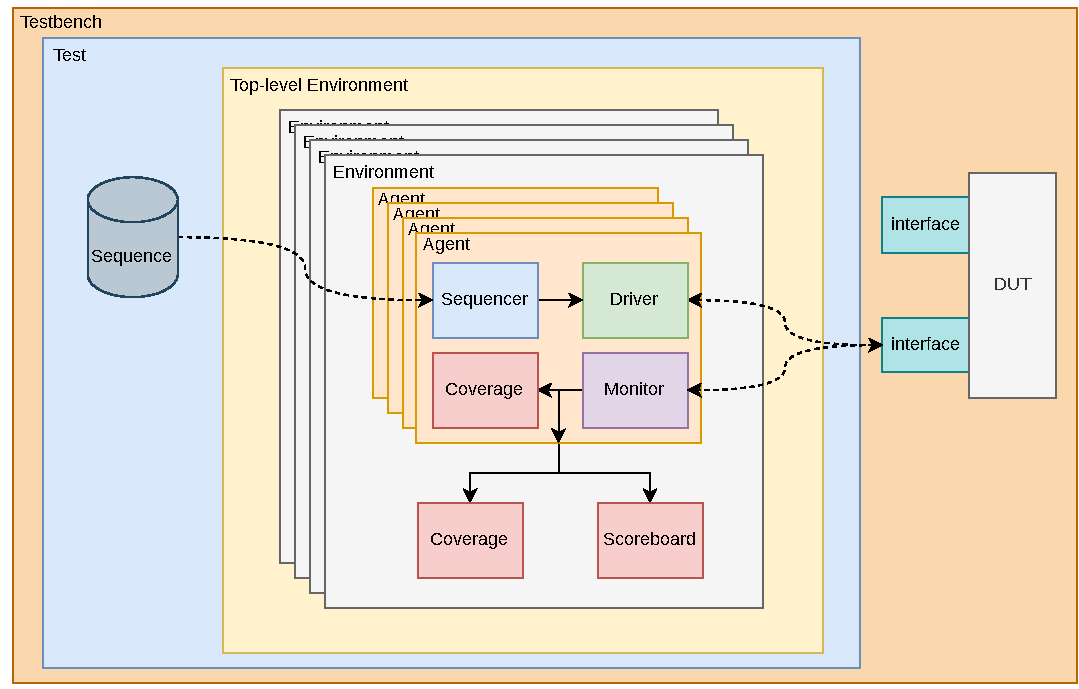
\includegraphics[width=\textwidth]{diagrams/uvm_structure.pdf}
\caption{The hierarchy of a simple UVM testbench.}
\label{fig:uvm_tb}
\end{figure}

The full UVM testbench hierarchy is presented in Figure \ref{fig:uvm_tb}. As it can be seen, in a complex system, the top-level environment itself consists of multiple other environments, which are specific for sub-systems of the DUT. Inside each environment, there are a series of agents which are specific to the interfaces which are part of the sub-system. Additionally, components collecting coverage information at the sub-system level may be present. Finally, the environment contains a scoreboard which compares the transactions observed on the DUT interfaces with transactions produced by some kind of model, the predictor.

An agent is specific to one interface, for instance AXI4 or SPI, and bridges the gap between the transaction level
and the driving and reading of the pins of the DUT. Agents come in two forms: passive and active. Passive agents only
observe transactions on the interface pins and send them to analysis components such as scoreboards or coverage
collectors. Active agents also accept transactions which they drive onto the interface pins. As it is shown in Figure \ref{fig:uvm_tb}, an active agent consists of a sequencer, a driver and a monitor. A sequencer serializes transactions from sequences and sends them to the driver, which applies them to the DUT through the use of virtual interfaces in SystemVerilog. The monitor observes the interface and converts the activity into transactions which are used by analysis components such as coverage collectors or scoreboards \cite[ch. 4.3]{mehta2018asic}.

\subsubsection{Communication between components} %----------------------------------------------------------------------------

The communication between the different components of the testbench is facilitated by the TLM (Transaction Level
Model) interface. The TLM is built around the idea of push and pull channels. The active side of a channel connection
(the producer in a push channel, the consumer in a pull channel) is called the \ttt{port} while the passive side is
called the \ttt{export}. The \ttt{export} provides a method for handling the receiving or sending of a transaction
which is triggered by the \ttt{port} \cite[ch. 4.5]{mehta2018asic}. 

Most of the time, two components are connected with a buffer between them such
that a buffered channel is created. In this case the buffer provides the two passive channel ends such that the
sender can call \ttt{put} at any time and the receiver can call \ttt{get} at any time. Calls to these methods are
blocking when no data is in the buffer. In the testbench, ports can be forwarded from a child component to a parent
component, exposing the port at a higher hierarchy level. This is for instance the case in an active agent, where the
port for the transaction stream to the driver is exposed by the agent itself. Next to single-producer-single-consumer
channels, the TLM also provides one-to-many channels with so-called \ttt{analysis\_port}'s. These are used to
broadcast transactions to multiple analysis components like coverage collectors or scoreboards \cite[ch. 4.5]{mehta2018asic}.

\subsubsection{Phases} %-------------------------------------------------------------------------------------------------------

\begin{figure}
  \centering
  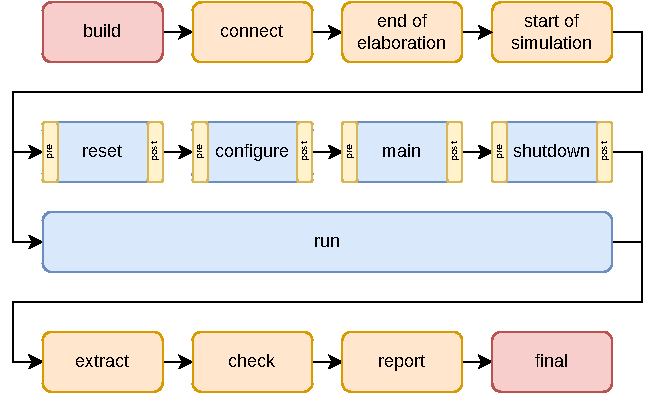
\includegraphics[width=0.7\textwidth]{diagrams/phases.pdf}
  \caption{Overview of the UVM phases. Top-down phases are red, bottom-up phases are yellow and the run phases are blue.}
  \label{fig:uvm_phases}
\end{figure}

Another concept introduced by the UVM are phases. Working with more elaborate DUTs with complex reset sequences, it
becomes natural to split the handling resetting the DUT from the actual test case. In a parallel system like UVM
where multiple components run concurrently, the challenge then is how the components should agree when the test case
starts. As another example, analysis components in the testbench need to know when the test case has finished in
order to generate summary statistics \cite[ch. 4.6]{mehta2018asic}.

UVM solves this synchronization issue by defining a series of phases with each component having the option run during
a phase by overriding a specific method. An overview of all UVM phases can be seen in Fig. \ref{fig:uvm_phases}. The
phases can be divided into three groups: build phases, run phases and cleanup phases. In the build phases, the
testbench hierarchy is set up. The \ttt{build} phase runs top-down through the hierarchy. Here all component
instances are constructed using the UVM factory and each component can configure its children by setting the
ConfigDB. The \ttt{connect} phase runs bottom-up and is used to connect the TLM channels between the components
\cite[ch. 4.6]{mehta2018asic}.

In the run phases, the actual test case is run and the DUT is stimulated. That means that these phases are the only
ones consuming simulation time, signified by the usage of \ttt{task}'s instead of \ttt{function}'s in SystemVerilog.
As it can be seen in Fig. \ref{fig:uvm_phases}, next to a series of fine-grained run phases, there is also the
\ttt{run} phase itself which spans the whole simulation. The most important run phases are \ttt{reset},
\ttt{configure}, \ttt{main} and \ttt{shutdown}. During the \ttt{reset} phase, the DUT can be forced into a known
state. The \ttt{configure} phase should be used to set up the DUT for the actual test case, e.g. by setting up
memories. The \ttt{main} phase is where the actual test is performed, i.e. the stimulus is applied to the DUT. The
\ttt{shutdown} phase can be used to wait for all effects of the applied stimulus to take place \cite[ch. 4.6]{mehta2018asic}.

As noted by the authors of \cite{dvcon2014reset}, reset behavior should not only be verified at the start of a test
but potentially also midtest in CRV test cases. The UVM does not directly prescribe a way to handle this, and altough
jumping between phases is possible, this poses the challenge of gracefully terminating the current phase in all
components. The authors propose a reset monitor which invokes cleanup hooks in all components when a reset is detected.

The cleanup phases in the UVM are used for analysis components to determine whether the test was passed successfully
and whether secondary goals such as coverage were met. The purpose of each phase in this group is very narrow and is
evident by the name \cite[ch. 4.6]{mehta2018asic}.

\subsubsection{Transactions} %-----------------------------------------------------------------------------

We have seen that the stimulus for the DUT is abstracted as transactions in the UVM. Transactions are passed around
the testbench through TLM channels, decoupling the actual data in the transactions from the static structure of the
testbench. But transactions rarely come alone. Usually, a series of transactions is needed to test a specific feature
of the DUT. These sequences of transactions should not be produced in the test case itself, since that would not
allow them to be reused across different test cases. Instead the test case should rely on predefined sequences of
transactions which it composes to achieve the desired stimulus \cite[Ch. 23]{salemi2013uvm}.

In the UVM, transactions are derived from the \texttt{uvm\_sequence\_item} base class. A sequence item consists of
fields, some of which can be randomized subject to constraints, which encode a transaction. Sequences of transactions
are derived from the \ttt{uvm\_sequence} base class. The resemble generators, as they can be found in Python or F\#,
where a code body is executed which produces an ordered sequence of items. In Python and F\#, the \ttt{yield} keyword
is used to produce items. In the body of a UVM sequence, the \ttt{start\_item} method synchronizes the sequence with
a potential consumer. A call to \ttt{finish\_item} signals that the item is ready and it is sent to the consumer. A
feature which is not a part of usual generators is, that the consumer can answer itself with a transaction of a
potentially different type to the transaction it received from the generator \cite[Ch. 4.3]{mehta2018asic}.

To maximize reuse, sequences should themselves be composable. Combining sequences should not be done by the test case
itself, since this would again not allow for reuse of the composed sequences. The UVM solves this by allowing for
so-called virtual sequences, which are sequences that "play" other sequences in their body. A test case can reference
such a virtual sequence instead of composing the individual sequences itself. The individual sequences in a virtual
sequences do not have to necessarily target the same consumers, which means that sequences can be sent to different
drivers in parallel. This allows for the encapsulation of cross-interface interactions with the DUV in a single
construct \cite[Ch. 23]{salemi2013uvm}.

One aspect which has not been discussed yet, is how the transactions actually enter the static infrastructure of the
testbench. Instead of being directly sent to a driver, transactions pass through a so-called sequencer in the UVM
before ending in a driver. When a sequence is started, i.e. it starts producing transactions, it is handed a
reference to a sequencer. The sequencer has a TLM port to which it forwards the transactions it receives from the
sequence. A sequencer can possibly receive transactions from multiple sequences at the same time, and it is up to the
implementation to arbitrate the order in which the transactions streams are merged \cite[Ch. 23]{salemi2013uvm}.

Sequences can be composed and run in parallel on multiple interfaces using virtual sequences. In this case the virtual sequence handles the coordination between the different transaction streams. Sometimes it may however be necessary to coordinate the transaction streams to multiple interfaces which originate from \textit{different} sequences. This could for instance be the case, if a timing relationship between handshakes on different interfaces is required. Here the UVM provides the concept of a virtual sequencer. It holds references to a set of actual sequencers and provides mechanisms to control them. Sequences, virtual or not, target their sequencers via the virtual sequencer which coordinates the interactions between the different interfaces \cite{virtualseq}.  

\begin{comment}
\cite[Ch. 23]{salemi2013uvm}
- in order to make testbench reusable, structure should be separated from data i.e. Transactions
- this also includes the stimulus that is the ordered sequences of transactions
- the ordered sequences could also be used across different test cases -> test case should not decide the specific transactions
- instead test case could operate on collections of transactions which are used like a library

\cite[Ch. 4.3]{mehta2018asic}
- sequence items are the base class for transactions in the UVM
- just class which consist of random and non-random fields with constraints
- sequences represent a stream of sequence items
- in the code they resemble generators
- a body method is invoked and new sequence items are produced as part of the sequence by calling a method
- a special thing is through that when a sequence item is produced, a response may also be obtained which could be another transaction type
- the start\_item method passes the reference to the sequence item to the receiver and waits until a receiver is ready
- when finish\_item is called, the receiver is informed that the item is valid and can be processed
- the sequence is paused until the receiver signals that it is done with the item and a response item may follow that confirmation

\cite[Ch. 23]{salemi2013uvm}
- but what if we want to compose sequences such that the combination is reusable
- can not be done in the test case
- instead a virtual sequence can be used
- it can play other sequences in its body
- sequences can be played in parallel and may be sent to different targets
- this gives control on how interactions on different interfaces are interleaved

\end{comment}

\subsubsection{Component Types} %----------------------------------------------------------------------------------------------


Now that the high level structure and way of functioning of a UVM testbench has been introduced, a more thorough description of the component types which play an active role in the testbench is given.

% driver
A driver has a port on which it can receive transactions. Normally, a driver enters an infinite loop in the \ttt{run}
phase where it wait for transactions and applies them either directly to the DUT or does so via a BFM. In order to
interact with the DUT, it is necessary in SystemVerilog to use a \textit{virtual interface} which effectively is a
handle to the pins of the DUT. The driver gets the next transaction through a call of \ttt{get\_next\_item} and
signals that the transaction has been applied by calling \ttt{item\_done}. The driver can provide feedback to the
code generating the sequence by passing a new transaction to the \ttt{item\_done} call. Special care has to be taken
when an interface is pipelined, i.e. when the DUT can accept multiple transactions before the first one is
acknowledged. In this case, the driver has to keep track of the transactions which are in flight and has to make sure
that the transactions are applied in the correct order \cite[ch. 4.7]{mehta2018asic}.

% monitor
A monitor holds, like the driver, a handle to the pins of the DUT. It observes the state of the pins and translates
the observed activity into transactions which are published via one or multiple analysis ports \cite[Ch. 4.3]{mehta2018asic}.

% subscriber
A series of subscribers can then receive these transactions and act upon them, for instance collecting coverage
information or comparing the transactions to a model. A coverage collector looks at the incoming transactions and
uses SystemVerilog functional coverage features to keep track of statistics such as whether a read was performed
after a write \cite[Ch. 4.3]{mehta2018asic}.

% scoreboard
The task of verifying that the transactions produced by the DUT are correct is handled by the scoreboard in the UVM.
The UVM does not prescribe a way of how exactly to achieve this. Since correctness has to be checked for an arbitrary
stream of transactions, some form of a model is usually needed. Depending on the complexity, this model could be
included in the scoreboard or be its own component which just like the DUT receives one or multiple transaction
streams and produces another set of transaction streams. The scoreboard is in this case reduced to comparing the
result streams of the DUT and the model \cite[Ch. 4.3]{mehta2018asic}.

\subsubsection{Configurability} %----------------------------------------------------------------------------------------------
%- Configurability
%  - factory
%  - configDB

The introduction of the component system, each with their well defined responsibilities, is only one part of the way
towards reusable and scalable testbenches. Not only concepts and abstractions are necessary, but also guidelines and
programming patterns for how the testbench code should be implemented. How can a specialized component be derived
from another for a specific test case? How can different versions of a component be easily swapped out? How can a
component implementation be made configurable in a way that also works well with derived components?

The answer to the first question is inheritance, which is available through SystemVerilogs OOP features. A component
can be derived from another and override methods to specialize its behavior. The answer to the question of how to
swap out different versions easily which the designers of UVM and its predecessors chose, is the factory pattern. In
a factory pattern, objects are not created through their constructor, but through a factory method which dynamically
determines which object to create, possibly based on a set of standardized parameters. In UVM, all UVM objects are
registered with a global factory. When a certain component A should be used instead of another component B, a factory
override can be issued, resulting in the creation of component A in all places where component B would normally have
been created. Of course A should be a subtype of B, such that A and B share the same interface. This allows for very
simples swapping out of components in a testbench without making the test code parameterizable with respect to the
different component implementations \cite[Ch. 13]{salemi2013uvm}.

Due to the global nature of the UVM factory, a one-siz-fits-all approach has to be adopted for what parameters may be
passed to the factory method. In the UVM, only the name for the object is given when an instance is produced:
\ttt{my\_class::type\_id::create("MyName")}. This raises the question of how to configure instances of UVM objects,
since it is impossible to pass parameters as it would usually be done in a constructor. The UVM solves this problem
with a configuration database, the so-called \ttt{uvm\_config\_db}, a global dictionary which is aware of the
component hierarchy in the testbench. One component can set a parameter in the configuration database and a
sub-component will be able to query the database for the parameter. In order to allow for a component to have
multiple sub-components of the same type with different configurations, the configuration database accepts a
hierarchical path when depositing a value in the dictionary. The deposited value will only be visible to the
referenced component and all its potential sub-components \cite{configdb}.

Together, the factory and configuration database provide the means for a test case to tailor the static testbench
environment to its needs. The factory is responsible for swapping out full implementations, while the configuration
database makes it possible to change the parameters a specific component works with \cite[Ch. 4.3]{mehta2018asic}.

\begin{comment}

- components are one step towards a reusable and scalable verification environment, providing concepts and abstractions
- but reuse and scalability also have to be tackled at the programming level

- not alone good enough to provide primitives
- we also need to concern ourselves with software design patterns to create resuable testbenches
- how do we swap out different implementations? -> factory
- how do we specialize an implementation? -> inheritance
- how do we make an implementation configurable? -> configdb

\end{comment}

\subsubsection{UVM Tests} %----------------------------------------------------------------------------------------------------

Now that the static infrastructure of a UVM testbench and the mechanisms for creating stimulus have been introduced,
all that is left for a complete testbench is the test case itself. The test case holds the actual purpose of why this
test is needed encoded in the stimulus stream it applies to the DUV. To achieve this, it creates an instance of the
top-level environment which will hold all the static testbench infrastructure. It may or may not configure the
environment such that it fits its needs. Then, the test case creates instances of relevant sequences and directs them
to the relevant sequencers in the environment. The checking of the DUV's behavior and other analysis tasks like
functional coverage collection are all handled by the static infrastructure of the testbench. The test case only has
to start the sequences and wait for the test to finish \cite[Ch. 4.3]{mehta2018asic}.

\subsubsection{Register Abstraction Layer} %-----------------------------------------------------------------------------------

Many designs today are rich in registers controlling the configuration and therefore the functionality of a DUV.
These configuration registers are usually attached to a bus and memory-mapped. A common task in setting up a test
case would be to set these registers to a specific state, which, with the tools presented up to now, would require
the use of sequences which target specific addresses through a bus interface. This can become a tedious task and a
abstraction of the interaction with the registers of a design would be useful.

The UVM Register Abstraction Layer (RAL) provides a standard way to abstract the registers of a DUV, independent of
the bus interface which is used to accesses them. A model of the registers inside the DUV is created using predefined
classes for fields, registers, blocks of registers but also memories mapped into an address space. These models can
be generated by commercial tools based on a description of the register layout \cite{uvm_ral}.

The accesses to the register model are either translated into actual transactions which are applied through the bus
interface causing side effects in the process, or they are performed through simulator specific backdoor accesses
which do not cause side effects in the DUV. The UVM also allows for configuring the model to a desired state before
committing it to the DUV in one go \cite{uvm_ral}.

The classes used to construct a register model capture detailed information about the registers, such as for instance
their accesses policies like read-only registers, but also more complex ones like writing a 1 to a bit to clear it.
This information is used to predict the result of a read or write to a register in the model, such that it stays
synchronized with the actual registers in the DUV without the need to use backdoor accesses in every register
accesses \cite{uvm_ral}.

\begin{comment}
  \cite{uvm_ral}
- many designs today are rich in registers controlling the configuration of the DUT attached to a bus
- a common task in a test case is to set these registers to a known state to test a certain configuration
- with the tools preseted up to now, we would have to use sequences with specific addresses and data to set the registers
- this is a very tedious task, and engineers would probably develope their own abstraction containing addresses of regs
- the UVM RAL provides a standard way to abstract the registers of a DUT, independent of bus interface
- a model of the registers in the DUV is created using predefined classes for fields, registers, blocks or memories
- accesses to the model are either translated into transactions on the bus or are performed through backdoor accesses
- thus model is connected to the actual registers in the DUV
- frontdoor access use transactions for access and cause sideeffects
- backdoor access uses simulator specific access methods and does not cause sideeffects
- also allows configuring the model with .set before commiting to DUV using .update

- register fields can have different access policies such as RO, RW but also special ones like write 1 to clear a bit
-

- models are usually generated from a register description language

-RAL is actually just a transactor system with a reg model to generate meaningful transactions
\end{comment}

\subsubsection{Utilities} %----------------------------------------------------------------------------------------------------

In addition to the core concepts and their implementation, the UVM also provides small utilities which are a part of
handling testbenches. This includes most notably a standardized reporting and verbosity system. Macros are provided
for infos, warnings, errors and fatal errors, which automatically annotate the message with the hierarchical path of
the component that issued it. At the end of running a UVM testbench, a summary of how many warnings and errors were
encountered is
provided to the user. The amount of information printed to the console can be controlled by setting a verbosity level
\cite[Ch. 19]{salemi2013uvm}.

Finally, the UVM provides many macros which simplify the writing of the test code and reduce the amount of
boilerplate code. For instance, each component should call the \ttt{`uvm\_component\_utils(name)} macro, which among
others takes care of the registration of the component with the UVM factory.

%\cite[Ch. 19]{salemi2013uvm}

\subsection{Open-Source Alternatives} %----------------------------------------------------------------------------------------

\todo{meta text}

\subsubsection{Cocotb} %-------------------------------------------------------------------------------------------------------

Cocotb is an open-source project under the FOSSi foundation, which focuses on providing a productive and
vendor-agnostic testbench framework for Verilog, VHDL and even mixed-signal designs \cite{cocotb}. Cocotb, short for
Coroutine-based Co-simulation Testbench, uses coroutines in python as an efficient way of having many simulation
threads cooperatively interface one simulation. Simulation events are modelled as asynchronous function calls which
can be "awaited", resulting in the waiting thread to suspend execution until the simulation backend triggers the event.

While taking advantage of the low learning-curve and rich library ecosystem of Python, Cocotb also suffers from the
drawbacks of python like the lack of static typing and the overhead of the Python interpreter. Due to its ease of use
and support for all major simulators, including commercial ones, Cocotb is a popular choice for a modern open-source
testbench framework. It does however not provide the infrastructure for building scalable and reusable testbenches
like the UVM does.

Due to its popularity, a series of other extensions have been developed around Cocotb. Examples are the
cocotb-coverage \cite{crvpython} and PyVSC \cite{pyvsc} libraries which both add functional coverage collection and
constrained random stimulus generation capabilities to a Cocotb testbench.

\subsubsection{Chiseltest} %---------------------------------------------------------------------------------------------------

Chiseltest was developed as part of the Chisel hardware construction language \cite{chiselpaper} and is a Scala-based testbench
framework \cite{chiseltest}. Due to a change in the Chisel compiler infrastructure, it has been recently deprecated,
but a replacement is under development by the Chisel community. While meant to be used with Chisel designs, Verilog
designs can also be included via Chisel. The number of supported simulators is more limited compared to Cocotb,
supporting only Verilator, Icarus Verilog and Synopsys VCS when using Verilog designs. Chiseltest is integrated with
the scalatest testing framework, which allows for an efficient way to organize and run tests.

Chiseltest provides a simple peek/poke/step interface to the simulation and allows for multi-threaded testbenches
using a fork-join model. However, it does not provide any
level of abstraction and infrastructure for building complex
testbenches, focussing on directed unit-test-style testbenches.

Work has been done on extending Chiseltest with formal verification features \cite{laeufer2021open}. This feature is deeply integrated with the Chisel hardware construction language and allows the user to write formal properties in the source code of the design in Chisel just like in SystemVerilog.

\subsubsection{ChiselVerify} %-------------------------------------------------------------------------------------------------

ChiselVerify is a verification library for Chisel designs built on top of Chiseltest \cite{chiselverify}. It aims to
improve the verification capabilities in the Chisel ecosystem by providing verification tools such as functional
coverage, constrained randomization and formal verification features. While showcasing how a BFM can be built using
scala and Chiseltest through a general AXI4 BFM, the framework does not provide guidelines and abstractions on how to
build standardized, scalable and reusable testbenches.

Functional coverage can only be collected at the IO of the DUT in ChiselVerify. It is not possible to collect
coverage at the transaction level which would require the monitoring of scala variables in addition to Chisel IO
ports. However, ChiselVerify allows for the expression of more complex cross coverage relationships. It not only
supports simultaneous hits between the cross-coverage bins but also timed relationships, for instance that a hit to a
bin results eventually in a hit to the crossed bin.

\begin{comment}

- functional coverage only on ports
- no sampling events for coverage
- but more complex timing relationship for cross coverage, i.e. not just simultaneous hits

- concerns itself with adding systemverilog verification capabilities
- does not provide methods to build reusable scalable testbenches

\end{comment}


\subsubsection{PyUVM} %--------------------------------------------------------------------------------------------------------

PyUVM is a project which aims to make UVM more accessible through the use of Python and by relying on open-source
tools \cite{pyuvm}. The project implements a subset of the UVM standard, which they describe as most frequently used,
in Python. As a motivation for implementing the project in Python, its ease of use due to light syntax and dynamic
typing are highlighted, and the existing verification infrastructure surrounding cocotb. The project tries to take
advantage of Pythons flexibility where possible to reduce the verbosity inherent in SystemVerilog. Among the UVM
features implemented in PyUVM are the factory, the configuration database, all component types, the TLM interface,
UVM phases, sequences and the register abstraction layer.

\subsubsection{UVM support in Verilator} %-------------------------------------------------------------------------------------

In addition to bringing modern verification features to new languages and environments to increase the accessibility,
work is also in progress to bring UVM support to Verilator \cite{uvm_verilator}. Verilator is a popular open-source
Verilog simulator which transpiles Verilog code to executable C++ models of the hardware design. The effort lead by
the Tools Workgroup in CHIPS Alliance aims to make Verilator fully capable of running UVM testbenches. In its current
state Verilator only supports a subset of SystemVerilog features. One crucial element is the addition of dynamic
scheduling in Verilator which is necessary for dynamically triggered events used in UVM. The effort of enabling all
SystemVerilog features required for a full UVM testbench is still in an early phase.

\section{Software Design Patterns} %===========================================================================================

\todo{meta text}

Software design patterns offer general solutions to reoccurring problems in software design. They provide
template-like solutions which prescribe a certain structure and organization of code. They represent a variety of
best practice approaches to software design. Design patterns can be grouped into three categories. Creational
patterns are concerned with making the instantiation of classes more flexible. Structural patterns are concerned with
the composition of classes and objects. Lastly, behavioral patterns are concerned with how objects communicate and
interact \cite[Ch. 1]{design_patterns}.

One creational design pattern was already encountered when discussing the UVM: the factory pattern. The factory
pattern decouples the decision of which object to create from the actual creation of the object. In place of the
constructor, a function is used which returns an object with a known interface. The function can be provided in two
ways. It could be provided by a so-called abstract factory, which is an object with an interface known to provide the
factory function. It could also be provided by a factory method, which derived classes implement to define which
object should be created \cite[Ch. 3]{design_patterns}.

A class C can be written purely relying on the factory for creating objects with interface L. The end-user has the
option to define what object with interface L should be created everywhere \textit{without} modifying the code for
class C. The factory does not have to be a global singleton as in the UVM, but could also be a parameter to the
constructor of class C. Furthermore, a factory is usually specific to a certain group of classes which share an
interface and common parameters. This is in contrast to the UVM, where one factory is used for all components, with
the only shared parameter being the parent component and the name of the component \cite[Ch. 3]{design_patterns}.

There are other creational design patterns which also facilitate the swapping out of different implementations of
interfaces used in a class. The dependency injection pattern relies on the user to actually construct the object it
depends upon and then provide them to the class through its constructor or setter-methods. The class works with the
object handel it has been provided, without knowing which concrete implementation of the interface it actually works
with. Unlike the factory pattern, no infrastructure for object creation is created, but instead the responsibility of
object creation is pushed up to the user of the class \cite{ioc_di}.

Another useful pattern is the observer pattern. It is a behavioral pattern, which is also known as the
publish-subscribe pattern. In a system where multiple objects, the observers, are interested in changes of the state
of another object, the subject, this pattern describes how observers should be notified. It is the subject which
maintains a list of observers and has the responsibility to notify them when its state changes \cite[Ch.
5]{design_patterns}. This pattern can be seen in the UVM where analysis components like the scoreboard or coverage
collectors are notified of transactions on the DUT interfaces through the monitor. In this case it is not directly a
change of state which the observers are notified about, but the occurrence of an event.

\begin{comment}

- factory pattern
- inversion of control and dependency injection \cite{ioc_di}
- service locator pattern
  - kind of like factory, an object know how to create the right other objects, if global singleton it its kind of like factory
- strategy pattern
- observer pattern

- publish subscribe pattern
- actor pattern \cite{actors}

\end{comment}

\begin{comment}

\section{Software Testing Methods} %===========================================================================================

\subsection{Unit Testing} %----------------------------------------------------------------------------------------------------

\subsection{Integration Testing} %---------------------------------------------------------------------------------------------

\subsection{Property-Based Testing} %------------------------------------------------------------------------------------------

\subsection{Black/Grey/White-Box Testing} %------------------------------------------------------------------------------------

\subsection{Fuzzing} %---------------------------------------------------------------------------------------------------------

\subsection{Mocking} %---------------------------------------------------------------------------------------------------------

\end{comment}

\chapter{Problem Formulation and Methods}
%///////////////////////////////////////////////////////////////////////////////////////

The UVM provides abstractions to compartmentalize a testbench in a standardized way. Instead of each engineer or
company defining their own abstractions, the UVM provides shared abstractions and a standardized application
programming interface (API). This makes it possible to quickly
understand an unknown testbench and to reuse parts of it in other projects. It also facilitates the exchange of
verification components between different entities and eases the hiring of new verification engineers.

However, the UVM is a complex and large framework. A lot of the literature on UVM focusses on how the UVM wants us to
build testbenches, but not necessarily why it was designed that way. Considering the process of its creation, it can
be seen that the UVM is something which grew
out of series of other methodologies and carries a lot of legacy with it. It seems the UVM always tries to anticipate
every possible use-case, leading to its size and complexity. It is therefore worth an investigation whether all of
its features are actually used in the industry and whether some of the features could be simplified.

While other open-source projects have explored bringing modern verification features like functional coverage,
constrained randomization and complex assertions to new languages, little concern has been given to how scalable and
flexible verification environments could and should be developed in the respective languages. Languages like Python
or Scala used in PyUVM or ChiselVerify bring more features to the table than SystemVerilog in terms of
general-purpose programming, but it is not clear how these can be taken advantage of to build scalable and reusable
testbenches. Could a productivity gain be achieved by adapting the concepts and abstractions of the UVM and their
implementation such that they better fit these high-level languages? Which parts of the UVM should be carried over to
such a revised and adapted methodology?

As such, it seems like there is a research opportunity to investigate the UVM, its design choices and its usage in
the industry in order to define a verification framework in a modern general-purpose language. There are two levels
to this process: on the one hand, the concepts and abstractions of the UVM have to be considered, and on the other
hand their implementation in SystemVerilog has to be examined. These considerations lead to the following research questions:

\begin{enumerate}
  \item Is everything in the UVM standard necessary and used by companies in the industry?
  \item Can the concepts and abstractions of the UVM and their implementation be condensed and simplified?
  \item Can the features of a modern general-purpose language be taken advantage of to build a more powerful and
    flexible verification framework?
\end{enumerate}

To answer these questions, the following methods will be used. First, a small survey concerning UVM and verification
will be conducted through informal interviews with a small number of companies in the Copenhagen area which use UVM
in their verification efforts. The goal of the interview is to get an understanding of how the UVM is received in the
industry, how and what parts of the UVM are used and what improvements the companies themselves could imagine. Taking
account the insight gained from the interviews, the UVM will be analyzed to identify the design decisions behind it
and alternative design choices will be reflected upon to synthesize a set of requirements for a verification
framework embedded in a modern general-purpose language. Finally, an implementation attempt will be made following
the established requirements to evaluate the feasibility of the proposed framework and its ease of use compared to the UVM.

\begin{comment}

- a lot of the literature talks about HOW the UVM does things, but not necessarily WHY
- I want to try to answer that

- UVM provides abstractions to compartmentalize a testbench
- the engineer would else have to make them up himself -> each engineer would invent their own methodology
- UVM provides a standard way of doing things
- makes it easy to understand an unknown testbench
-> communication is also a big factor of why a methodology should be adapted

- can concepts in UVM be condensed/simplified?
- is all of UVM used/necessary for modern verification?
- is there a productivity gain in embedding a HVL as a DSL in a modern general-purpose language?
- what featues should such a model HVL DSL have?

- UVM seems to attempt to anticipate all possible use cases, but does not achieve this
- shouldn't a framework facilitate the most common use cases and offer a way of extending it for the less common ones?

method:
- informal interview with relevant companies in the industry from the copenhagen area
- look at other modern verification frameworks
- other published sources critically analyzing UVM

\end{comment}

% talk about company interviews
\chapter{Industry Survey} %////////////////////////////////////////////////////////////////////////////////////////////////////

\todo{meta text}

\section{Interview Outline} %==================================================================================================

The interviews were conducted relatively freely but with a set of questions in mind to guide the conversation. The
interviews started off with a set of questions about the company itself. This concerned facts like the size of the
verification department or the usual size and application of projects. The conversation would then move on to their
verification pipeline, starting from the specification to the tape-out. The tools used in the process would be
discussed alongside the verification methods employed. Of special interest was the fact whether the company had or
could consider open-source verification framework alternative like for instance cocotb. One area of interest was
whether any industry standards for testing like ISO standards were directly impacting the verification work. The
different levels at which a system were tested and their usage of reference models would be discussed.

From here, the interview would move on to UVM-specific questions. It would be discussed which features were used, how
well the reuse mechanisms were working and whether external verification IP (VIP) was used. Features like UVM
phasing, configurability mechanisms like the configuration database and the UVM factory would be discussed. Room for
criticism of the UVM would be given, and the interviewee would be asked to point out any limitations they had encountered.

The interview would then move to a general critical perspective, considering things like bottlenecks in the
verification process, unique issues the engineers had encountered and what they wished to see in future developments
in the verification area.

\begin{comment}
# General Questions

Verification Pipeline
- describe the general flow of your verification process from spec to signoff
- what are the interactions with the design team?
- do you use UVM

Automation
- have you integrated any automated tools or scripts into your verification flow to speed up repetitive tasks?

Standards
- Are you following any standards (e.g. ISO) in your verification process? If so, how do you ensure compliance?

Verification IP reuse
- how do you reuse VIP going from specification models to rtl to netlists
- do you develope your VIP inhouse or do you also obtain external VIP
- UVM is about reuse, how successful have you been in reusing components across different projects? And what difficulties have you encountered?

Special DSP needs
- have you done any special customization on top of UVM for DSP verification?

Verification methods
- how much do you use formal methods
- how do you define which parts to test using formal methods and which parts using simulation based methods

Tools
- which eda tools are you using
- have you looked at alternative frameworks like cocotb in python?
- cosim vs. compiled in SystemVerilog
- what is your opinion on integrating verification language with rtl language?

Test scales
- do you use different approaches for testing smaller design units

Coverage
- what coverage metrics do you use? Code coverage?
- what are the most important coverage metrics for you?

Debugging & verification
- how do you use your verification environment for debugging?
- do you use interactive running of testbenches?

Golden models
- how do you consrruct scoreboard?
- what do you put in your scoreboard?
- is it always a cycle/transaction accurate model?

Bottlenecks
- what are the biggest bottlenecks in your verification process? How do you address them?

# UVM Specific Questions

Phasing
- which phases do you use apart from uvm standard phases
- have you added custom logic to different phases

Configurability
- how satisfied are you with the configuration mechanisms in UVM
- how much do you use the configDB and uvm factory
- what would be the advantages over using formal parameters and generic class instead

Reuse
- how extensively do you use more complex inheritance to allow for reuse

# Open criticism

Criticism
- what limitations of uvm have you encountered
- Are there any language limitations that you encounter while developing your verification environment? If so, how do you work around them?
- did you have any use case where you needed to adapt your verification methods?
\end{comment}

\section{Company 1} %==========================================================================================================

Company 1 develops ASICs for the hearing aid industry, with a team of 7-8 dedicated verification engineers. The
verification tasks they are performing do not need to adhere to ISO standards directly, but these standards are
already captured in the verification plan. The company prefers using a single language for design to enable
incremental compilation and simplify the workflow. All verification IP (VIP) is developed in-house and actively
maintained, with reuse being a key focus across projects. Examples of reusable VIP include agents for standard interfaces like
APB and SWD. Additionally, they integrate models for external IP, such as EEPROM, using C or Verilog models. Reuse is
made easy and encouraged by maintaining a single code base for everything.

Once the specification for a new project is complete, verification begins in parallel with the design process. The
basic layout of the testbenches can be created early on, based on the interfaces being used. The company uses
module-level testbenches before moving to verification of the top-level. They make extensive use of different UVM
runtime phases, particularly reset phases, to improve modularity and composition. Over time, they have developed
their own standard scoreboard implementation and rely on the configDB to pass data between agents. Connectivity
checks are performed to ensure that specific configurations correctly link different parts of the design.

Their coverage strategy prioritizes functional coverage and FSM code coverage. Debugging is supported by
assertion-based verification, with assertions used for runtime checking, formal checking, or both. Debugging remains
an unpredictable part of the development process. Known bugs are particularly difficult to work around while trying to progress.

For simulation, the company uses VCS and employs continuous integration (CI) to manage regression testing. Each
regression run includes approximately 6000 simulations, with a total runtime of around six hours. Synthesis is also
performed as part of the regression flow, and coverage checks are automatically executed. The CI system ensures that
a freshly checked-out version of the project always works. Although they have considered PyUVM as a potential tool,
they find the speed insufficient for their needs. Furthermore, they are cautious about adopting new or niche tools,
fearing that it could complicate future recruitment efforts.

The testbenches of the company rely heavily on CRV. However, signal data streams are not purely random, but instead
they use typical data encountered in real-world scenarios, because change throughout time is difficult to capture in
constraints. To support DSP verification, MATLAB models are integrated into the verification environment.

The company is overall satisfied with their usage of UVM, but pointed out some shortcomings. Specifically, they
believe that code using the UVM factory is difficult to debug and maintain, while the register abstraction layer
(RAL) in UVM is incomplete. For instance, a single register block cannot be mapped into multiple address spaces, so
they developed their own extension to address this limitation. Concerning the UVM factory, they note that using
callbacks, a feature not available during the development of UVM, would be the better option to keep dependencies
modular in the code. They also observe that many UVM examples available online are outdated and focus only on trivial
cases. Additionally, they note that UVM was influenced by several companies of which some insisted on incorporating
features from their own verification methodologies, sometimes resulting in unnecessary complexity. While they
continue to use UVM, they are not opposed to a framework with fewer options and simpler design choices. They
also emphasize that power-aware verification remains a significant challenge.

In terms of recruitment, the company intentionally avoids using all UVM and SystemVerilog features to make hiring
easier. They believe that limiting the use of overly complex or non-standard features lowers the learning curve for
new engineers. They have observed that it is rare for software engineers to transition into verification roles, so
they do not see a need to tailor the verification environment specifically for software engineers. To further ease
the process of setting up a verification environment, they use a setup framework that can automatically generate the
basic structure for testbenches and unit tests.

One of the key challenges they face is that the test plan often becomes a bottleneck, more so than the actual
development time for testbenches. While development time tends to be predictable, debugging remains highly
unpredictable, especially when working around known bugs while trying to progress the verification effort.

\begin{comment}
Company 1 develops ASICs for the hearing aid industry.
- 7-8 dedicated verification engineers

- do not use all UVM and SystemVerilog features
- try to stick to standard features to make hiring easier
- develop all VIP inhouse
- reuse inhouse VIP across projects, e.g. interfaces like APB or SWD
- integrate C or verilog models for bought IP like EEPROM
- use VCS for simulation
- prefer single language for design to enable incremental compilation
- think that register abstraction in UVM is very complex
- have testbenches at the module level
- use randomized inputs (CRV)
- integrate matlab models for DSP
- Signal data streams are not random but represent typical data
- constraints in time, i.e. between signal packages, are difficult
- use FSM code coverage
- no line or branch coverage
- functional coverage

- after specification is finished, verification starts in parallel with design
- basic testbench layout can be created based on interfaces

- for debugging, assertion-based verification is used, some formal, some runtime, some both
- use connectivity checks to check that certain config connects certain parts of design

- for regression CI is used
- checkout always works
- 6000 simulations with tests
- 6 hours runtime
- synthesis is also done for regression
- coverage checks are performed

- no ISO standards have to be considered by the verification team
- standards are required for chip set, already captured in verification plan

- inhouse VIP is actively improved and maintained and reused
- 1 code base for everything

- have looked at PyUVM but speed is an issue
- want a setup framework to generate basic structure of testbench
- want a setup framework to generate basic unit test structure
- afraid of adapting new niche tools since it may be a recruitment issue

- in their experience it is rare that software engineers become verification engineers, do not see need to tailor verification environment to software engineers

- prefer formal methods over unit tests

- in terms of bottlenecks, the testplan is more of an issue than the actual development time of the testbenches
- Development time is also more predicatable, debugging is not
- especially working around known bugs to further progress is difficult

- use the different UVM runtime phases extensively, especially reset phases, to increase composition
- UVM factory is difficult to debug, and hard to maintain
- callbacks would be the bettern option but were not available when UVM was drafted

- have their own standard scoreboard implementation

- UVM is not perfect, some companies insisted on things from their own methodology

- use configDB to pass data to agents

- RAL is not finished in their opinion
- e.g. one reg block can not be mapped into multiple address spaces
- developed their own extension

- UVM examples on the internet are often outdated
- only showcase small and trivial examples

- power aware verification is still difficult

- like idea of a framework without too many choices
\end{comment}

\section{Company 2} %==========================================================================================================

Company 2 offers consulting services for hardware design and verification, including training for UVM, thus bringing
extensive experience in handling various verification challenges.

Verification at its core is about building confidence in the design in their opinion. The process typically follows
an evolutionary path: initially, few bugs are found, then many bugs surface as the verification infrastructure
matures, and finally, the design stabilizes with no remaining bugs. This approach often involves dividing the
verification task into smaller, manageable features and verifying them separately. Effective verification requires
robust coverage models, as weak models give misleading results. These coverage models can be validated through
intentionally weak tests, which are expected to score low. However, it is important to note that coverage only
accounts for known-knowns and known-unknowns; there is no established methodology for addressing unknown-unknowns,
i.e. bugs that are not detected by the verification plan. The company follows the best practice of always capturing
design assumptions in assertions.

Formal verification is considered a superior tool for proving design correctness by the company but often struggles with the
complexity of large designs. Despite these challenges, formal methods remain a critical component of their verification process.

They perceive UVM to be a well-working tool for verification. Like all tools, it is not perfect though, and they note
some small issues which they have encountered. The ConfigDB mechanism, can confuse users, in their experience, due to its
hierarchical scoping mechanism. Misunderstanding its usage can lead to spaghetti code, but when used correctly, the
ConfigDB solves the essential problem of enabling communication between classes without direct references. It acts as
a middleman, allowing information to be passed down from the test to the environment, agents, and drivers. Sometimes
they even use the ConfigDB as a channel, where a driver monitors specific keys for changes to receive data.

They note that the UVM factory mechanism generally works well for flexible component creation. In object-oriented
programming with static hierarchies, the creation of many small specific factories for component substitution in the
hierarchy would be necessary anyways. UVM's global factory addresses this need, reducing the programming overhead for
the end-user. But the UVM factory also introduces overhead, due to the indirection of object creation. Best practices
include using direct instantiation when no overrides are expected or limiting factory use to scenarios where dynamic
changes are really necessary.

Phasing in UVM works well for the company. But there are some issues concerning the communication of phase
completion. Each component can stop the phase from completing by raising an objection. However, this can lead to
problems when the main test code finishes injecting stimuli while the testbench still has to wait for responses. The
UVM predecessor VMM had a consensus object that allowed components to register their “done” conditions, offering a potential
solution. In agents, reset should be handled within the run phase. Base tests should handle reset and shutdown
phases, while derived tests should handle configuration and main phases. The company has developed its own standard
scoreboard infrastructure, which focuses on comparing streams of transactions.

They note that the Register Abstraction Layer (RAL) poses several challenges. It assumes a direct mapping of one
register transaction to one bus sequence item. This assumption can be problematic when protocols require multiple
transactions to complete the changes implied by the register transaction. Additionally, while the RAL supports
writing individual fields, certain protocols do not support this and would need a read-modify-write cycle, resulting
again in multiple sequence items. Locking registers by calling \ttt{.lock()} is available but does not ensure
immutability, raising questions
about its utility. Register randomization can be achieved using the `rand` keyword on fields, but unlike read/write
operations, calls to `rand` are not synchronized if multiple components access the register model in parallel. There
are currently multiple ways of injecting constraints into the register model, but none of them work well or are
verbose according to the company.

Certain types of DUTs present unique challenges. In a scenario where a DUT processes a stream, the interface where
the input stream is consumed may be separated from the one where the output stream is produced. This means the
resulting processed stream items flow though a different agent than the input stream items. An issue arises, if the
test case would like to make a decision based on the processed stream. The test case can only receive feedback from a
driver that it has sent a transaction to. In this case, it would like to receive feedback from a completely different
agent. This case is not considered in UVM. A solution was outlined, where the agent receiving the processed stream
would receive dummy transactions from the test case, such that it could answer with items from the processed stream.

DUTs that only produce outputs, such as random number generators, pose another issue: determining when to stop the
test. Timing-related challenges also arise when one has to determined whether transactions occur simultaneously
across multiple interfaces. The analysis ports of all interfaces would have to send either data or null each clock
cycle, reducing significant overhead, if this was to be determined. Another issue revolves around DUTs like filters,
which require initial stabilization before producing valid output. This could be handled by using metadata in
transactions or RTL signals to indicate readiness.

The company is satisfied with commercial verification tools, but they note that access to these tools remains a
challenge in educational settings, where they are typically available only during courses. They believe that this
educational space should be filled by open-source alternatives such as PyUVM, which they are actively exploring.

\begin{comment}

Company 2 offers consulting services for hardware design and verification, including training for UVM.

- one issue with the RAL is register randomization, they have their own implementation
- scoreboard: have their own standard scoreboard implementation
- model is not in scoreboard, scoreboard only compares streams of transactions

- first step is usually systemC model which can also be used for firmware development
- verification is about model checking
- assertions are alos a model
- verification process is about building confidence, first no bugs, then a lot, then no bugs again
- as verification infrastructure improves, the number of bugs found increases

- UVM falls apart in multi-clock designs

- assertions should be close to the interfaces

- a VIP should already contain a coverage model
- for system level coverage, cross coverage between different agents can be used

- coverage model has to be good, otherwise it is not useful
- can be check with intentionally weak tests

- design assumptions should be captured in assertions

- assertions have to be back-annotated to specification

- verification engineer also has implicit assumptions about how to attack the problem of proving that something is correct

- coverage only contains the known-knowns and known-unknowns
- no methodology to find unknown-unknowns

- for companies, the commercial tools are fine
- they see problem for education, where access to the commercial tools is only available during the course

- verification is about confidence in the design
- divide and conquer, by splitting into features and verifying them separately

- configDB often confuses people due to the scoping mechanism
- can lead to spaghetti code, if one does not know what they are doing
- but it solves one essential problem: talking to a class you do not know
- allows communication between two classes without them holding a handle to each other
- configDB is the middle man
- maybe it would be a good idea to have a configDB without scoping, too
- config is passed down from test -> env -> agents -> driver
- sometimes use configDB as channel -> driver monitors configDB for changes at a certain key

- satisfied with UVM factory
- in OOP program a static hierarchy exists
- if you want to change out components in the hierarchy, you would build your own micro-factory anyways
- why not have a global real factory
- factory comes with overhead though, so use new when it is known that no override will occur
- or limit construction to those times strictly necessary, e.g. at an actual value change

- phasing is a good idea
- reset and shutdown should be provided by base test
- config and main phase should be provided by the derived tests
- agents or any other component should only have a run phase
- one issue is the communication of when a phase is done
- raise and drop objection is used
- but sometimes the test code is done injection stimulus, but the TB should wait until all responses have been received
- VMM had a consensus object where objects register a "done" condition

- in an agent, the reset should also be handled in the run phase

- the scoreboard is application specific, but the infrastructure can be generalized
- this was presented in a paper at DVCon

- one issue is reactive slave
- DUT with interface to producer and consumer, consumer agent should be passive
- but what if test case needs access to values received by consumer?
- need to make consumer active and send one seq item per value, to get feedback
- can not use objections here, else you get stuck

- another issue are DUTs which only have outputs, like an random number generator
- how to know when to stop the test?

- another issue is timing related: when do transactions actually happen at the same time?
- for instance a coverage collector listening to 3 interfaces and should only sample if transaction at the same time on all three interfaces
- in current UVM, monitors would have to send null or transactions every cycle

- another issue are DUTs like filters where some data is needed for the DUT to stabilize and produce valid output
- could use meta data in the transaction
- could also use RTL signal as event to signal that the DUT is ready

- RAL is very big, 25\% of UVM class description
- can write fields individually, what if protocol does not support that? Would need read-modify-write cycle on the bus
- assumes mapping of one register transaction to one bus sequence item, what if multiple are needed?
- should allow translation of register transaction to sequence of bus transactions
- registers have a lock method, but that does not mean they are immutable, why is this there?

- randomization of registers can be done by using rand keyword on fields
- calls to rand are not synchronized though, in contrast to read and writes to the register model
- difficult to inject constraints into register model, without being verbose
- also difficult to randomize only one specific reg -> DVCon paper

- general perspective
- verification progress is not linear -> sometimes hard to communciate between engineers and managers
- the spec is not always perfect
- sees hope in AI DSL for spec
- formal is the better tool, but struggles with complexity

\end{comment}

\section{Company 3} %==========================================================================================================

Company 3 develops ASICs for the hearing aid industry. Their verification team consists of two dedicated engineers,
though verification responsibilities are shared with design engineers. Design engineers handle simpler verification
tasks, while the verification engineers focus on more complex aspects. The company follows a waterfall development model.

About six years ago, they transitioned to UVM and have since adopted a standardized subset of UVM to ensure
consistency across projects. Agents are frequently reused since most projects rely on the same interfaces. Their
Testbenches are employed not only for functional verification but also for gate-level simulations. While external
VIPs have been used and integrated successfully, most VIPs are developed in-house. Formal methods are used mostly for
their to application-specific instruction-set processors (ASIPs), but outside of that, formal verification is used
only in cases where it is easily applicable.

Their verification framework includes both module-level and top-level testbenches, with UVM environments from the
former being reused in the latter. They also maintain a basic test framework for simpler verification needs. The
employed reference model are mostly transaction-accurate and Matlab models are used for verifying DSP blocks.

The company uses code coverage, but mainly focusses on functional coverage. Like in Company 1, CRV is used except for
the modelling of audio streams where representative data streams are used instead. They note that debugging is one of
the most time-consuming parts of the verification process, often taking up to 70\% of the overall verification effort.

The team makes use of all UVM run phases, setting up the DUT and handling all analysis during the appropriate reset,
configuration and shutdown phases to simplify the work of test case developers. They find the UVM Config DB effective
for parameter passing, in part because they view parameterization of classes in SystemVerilog as cumbersome. Over the
years, they have developed their own UVM extensions, including a custom scoreboard implementation. One issue they
note concerning phasing is the handling of reset during the test. A solution is to do phase-hopping to go back to the
reset phase, which is a messy solution according to them.

Rather than seeing limitations inherent in the UVM, they see more limitations in SystemVerilog itself. For instance
parameterized interfaces can cause issues, and the language's verbosity and boilerplate code could be improved
according to them. Clocking blocks are also avoided due to frequent problems with multiple driver conflicts. While
they generally have no issues with the UVM factory, they believe it would be helpful if unsuccessful overrides
specified via the command line generated explicit error messages. The UVM factory is primarily used by the team to
adjust constraints and replace general sequences with more specific ones when necessary.

Overall, the team places a high priority on maintaining clear and understandable verification code, particularly so
that RTL engineers can easily work with it, too. They prefer straightforward, maintainable code over overly complex
features such as event callbacks.

\begin{comment}

Company 3 develops ASICs for the hearing aid industry.

- 2 dedicated verification engineers

- work in waterfall model
- verification engineer only involved in complex verification tasks, else design engineer does verification

- ISO standard requirements are already encoded in verification plan

- switched to UVM around 6 years ago

- many interfaces are repeated, agents can be reused

- reuse testbenches also for gate level simulation

- have used external VIP, was easy to integrate
- but many develope their own VIP

- there is a "standard" UVM subset

- CRV not used for data audio streams
- coverage is important though

- use code coverage, but disable it for some parts of the design

- use formal methods especially for their ASIPs
- else use formal only in obvious cases

- have their own basic test framework
- module level + top level testbenches
- UVM environment from module level testbenches is reused in top level testbenches

- reference models are cycle or transaction accurate
- some matlab models generate RTL -> model comes for free

- bottleneck is verification, around 70/%
- but out of this, debugging takes the longest time
- soemtimes need to argue why error is actually not an error
- communication overhead and manpower

- use all UVM run phases
- set up everything behind the scenes for the test developer

- config DB works well for them for passing parameters
- thinks that parameterization of classes does not work well in SystemVerilog

- clocking blocks offen suffer from multiple driver problems, because the tools can not understand them
- tend to not use clocking blocks

- does not see a problem with the UVM factory
- only unsuccesful overrides through CLI do not give errors, but should
- are used to change constraints
- used to replace general sequences with specific ones

- have own UVM extensions and methodology
- have own scoreboard implementation

- one issue is reset handling in CRV
- own agent for reset handling
- phase hopping is difficult and messy

- see most issues with SystemVerilog limitations
- parameterized interfaces
- verbose
- boiler plate

- but prefers guidelines over limitations for UVM

- prefers to keep verification code simle and understandable, also for RTL engineers
- does not like overly complex features like event callbacks

\end{comment}

\section{Takeaways from the Industry Survey} %=================================================================================

In general, companies seem to be satisfied with what the UVM can offer them. They acknowledge that it may have some
shortcomings, but it is an industry standard which most importantly is supported by all major EDA vendors, saving the
companies from the infamous vendor-lock. Having a standard also eases the hiring process, since new employees knowing
UVM can more easily understand the existing infrastructure.

It is also clear that only a subset of all the functionality which UVM offers is actually used by the companies. This
subset seems to consist of the core ideas behind UVM and seems to be generally accepted. Where UVM does not satisfy
their needs, companies have gone to implement their own extensions like for the scoreboard of the register
abstraction layer. This of course partially defeats the purpose of UVM, but is also a product of the universalism of
UVM, where abstractions have to fit all use cases and thus may need extra work before being able to be used for any
of those use cases.

Although formal methods are acknowledged as superior, allowing quick and exhaustive checking of a certain feature,
all companies only use it where the performance of current tools allows them to. Dynamic verification is thus still
highly relevant and the reusability mechanisms in the UVM seem to be appreciated and used by the companies to lower
the effort of developing new testbenches.

Some companies note languages limitations in SystemVerilog itself which proves the point of investigating
verification frameworks in more powerful languages. Due to long simulation times for their tests, performance is of
concern though, and has inhibited the use of co-simulation frameworks like cocotb in the production environment. Also
compilation times seem to be an issue for some companies.

As it can be seen in the example provided by Company 2, UVM is not perfect in facilitating dynamic tests, where the
test case produces stimuli as a reaction to the DUV's responses when these are spread over different interfaces. The
model of how the test case can get feedback from the DUV should therefore be investigated.

The opinions on the UVM factory differ, with some companies seeing it as a key part of creating flexible testbenches
and others seeing it as the source of hard to debug errors. It could be interesting to investigate what other options
exist and how user friendly they are.

The RAL seems to be a common point of criticism, with all companies pointing out that it has some issues. This should
also be investigated.

\begin{comment}
- companies are generally satisfied with UVM
- they see it as a tool which may have some shortcomings but it is a standard which is supported by all 3 major EDA vendors
- they only use a subset which seems to be generally accepted across the industry
- where UVM does not satisfy their needs, or does not specify a specific way of handling something (like scoreboard),
they have developed their own extensions

- compilation times seem to be an issue for some companies

- the approach of having IP units per interface seems to work well, and encourages reuse

- the phasing system seems to be good to facilitate composability of test scenarios

- although formal methods are acknowlegded as superior, where they work, they can not be applied to verify all parts of
a design and a simulation based framework is still needed

- There are different opinions on the UVM factory, it could be interesting to investigate what other options exists
and how user friendly they are

- all agreed that the RAL has some issues
- especially the mapping of one register transaction to one bus sequence item is problematic and easily addressed

- some point out that SystemVerilog itself limits what UVM can do, so it could be interesting to investigate what
other languages could do in the context of hardware verification
- performance is of concern though

- there seem to be some issues related to how the test case code gets feedback from the testbench in order to write
interactive test case code
\end{comment}

\chapter{Analysis and Design}
%///////////////////////////////////////////////////////////////////////////////////////////////////////////

\todo{meta}

In this chapter, ideas for a verification framework embedded in a modern programming language will be developed based
on the understanding of existing tools and frameworks as well as the insights gained from the industry survey.

\begin{comment}
- here, the requirements should be made and possible approaches outlined
- this includes possible tools to rely on (also for features which are not part of the final product, e.g. coverage and crv)

- there are two levels to the design:
- the concepts, abstractions that the testbench is strucured by
- the coding principles which facilitate the flexible nature of the testbench

story:
- first define the scope of this project
  - we look at UVM features as the current status quo and evaluate them and if they are considered useful, determine how to be integrate them into a new framework
- then some basic decisions have to be made since they limit the design choices
  - the simulation backend has to be chosen
  - the verification language has to be chosen
    - should it be a embedded DSL or a dedicated Language
    - reflection should be made even though the answer is clear -> DSL is the only realistic path
    - here the approach using CIRCT should be mentioned
- having established the basic infrastructure, the requirements can be made
- first the basic simulation infrastructure has to be established
  - how should the simulation be interacted with?
    - what kind of data types are necessary to interface with the simulation?
    - how should the interface be captured in the DSL?
    - what actions can be performed on the interface?
    - what are the timing semantics? clocks and steps
    - timing resolution?
    - concurrency -> the simulation thread
    - thread interaction with simulation
    - interthread interaction
    - test entry point
- then the test bench abstractions and concepts should be defined
  - what phases does a test bench have?
  - what are the basic components and the basic structure of a test bench?
  - how are test cases defined?
- then design patterns for reuse should be defined
  - how can components be swapped out?
  - how are components configured?
\end{comment}

\section{Scope} %==============================================================================================================

First of all, a overall scope for the verification framework has to be outlined. The goal is to develop a
verification framework which is embedded in a modern programming language and which takes inspiration from UVM for
reusable testbenches. The framework should provide a set of features such that it could be used instead of
SystemVerilog and UVM for the development of testbenches.

At its core, the framework has to provide a simulation interface in order to allow the user to interact with an
instance of the DUT. The simulation interface should allow for multiple threads to control and access the DUT
concurrently. The tool responsible for simulating design should support general RTL designs.

A modern testbench would not be complete without a way to generate constrained randomize and collect coverage
information. As such, mechanisms for both features in the language of choice should be provided. \todo{but since this
  has been explored in python and scala already, not of concern for me, but a small consideration of how it may be
integrated will be made}

The previous requirements provide the foundation for constructing testbenches. To facilitate the development of
reusable testbench infrastructure, the framework should provide a set of primitives similar to those found in the
UVM. This includes some form of verification base components responsible for different tasks in the testbench, a
phasing system to structure the testbench execution and a way to organize stimulus into sequences. All these features
should be easily composable into testbenches and test cases.

\todo{should functional coverage and crv be considered outside of the scope from the start? But why talk about them
in the background then. Maybe they can be described more shallow}

\todo{while allowing for the development of complex testbenches ala UVM, the framework should also aim to simplify}

\todo{what parts of UVM should be integrated?}
- here \cite{sutherland2015uvm} can give an answer
- it describes a practical subset of UVM which allows to construct UVM testbenches
- it acknowledges that UVM has a lot of redundant features and features which are only useful in rare cases
- it recommends a subset of UVM as a quick way to exploit the benefits of UVM
- this shall be the basis for the integration of UVM features into the new framework

\todo{elaborate}

\begin{comment}
- a library of primitives for reusable testbench infrastructure

- purpose: ideas for a verification framework in a modern language which takes inspiration from UVM for reusable testbench components and could provide a replacement for SystemVerilog+UVM
- not all features will be implemented necessarily
- on the one hand, a simulation framework for hardware designs
- should be multi threaded
- the level of simulation depends on the backend (for instance 4 state logic)
- could be its own language,but this would be too complex for the time frame
- instead an embedded dsl should be used
- a modern language should be used

- simulation framework should feature coverage collection integrated with simulation backend for sampling
- should feature constrained randomization library for random objects

- on the other hand, primitives for a reusable testbench environment should be provided in a library
- there are two levels to this design process:
  - the abstractions and concepts
  - the coding principles which facilitate the flexible nature of the testbench
- it is clear that the coding principles are deeply interwoven with the implementation
- this includes some form of verification components responsible for different tasks in the testbench
- some kind of phasing system should be designed to compartmentalize the execution of the testbench
- some form of organization of stimulus into sequences should be provided
- a easy interface for running tests should be provided
\end{comment}

\section{Verification Language} %-------------------------------------------------------------------------------------------

The first choice to be made is, which language the verification framework should be integrated into. On the one hand,
this can be seen as an implementation choice, but on the other hand, the chosen language may limit the design choices
in terms of capabilities and syntax. Therefore the decision is made prior to designing the functionality of the
framework. The examples
which have been discussed were cocotb and PyUVM using Python, but also Scala being used by Chiseltest and
ChiselVerify. Before reflecting over these languages and other options, it is also worth considering the advantages
and disadvantages of embedding a verification framework into another language compared to developing a standalone
language such as Vera or even integrating it into the design language itself such as it is the case in SystemVerilog.

One of the primary advantages of embedding a verification framework into a general-purpose language instead of
developing a standalone hardware verification language or a shared design and verification language, is the effort
associated with developing all the necessary tools and infrastructure. A standalone language requires its own
compiler or interpreter which will have to be maintained. Any additional functionality which is not part of the
language itself has to be developed from the ground since no library ecosystem exists, as it is the case for
general-purpose languages. Additionally, many modern languages provide a dependency management system, which can be
leveraged to share and reuse code. Finally, quality of life features such as IDE support of the host language can
also be leveraged.

When performance is considered, a combined design and verification language has a clear advantage, since everything
can be compiled and optimized together. In a standalone language or an embedded language, a simulation has to be
interfaced by a runtime. Depending on the implementation, this can lead to a significant performance overhead.

When it comes to ease of use and the learning experience, dedicated languages have the advantage of being able to
tailor their syntax to the domain, making it easy and concise to express the concepts of the domain. On the other
hand, a whole new syntax has to be learned, which can be a hurdle for new users. For an embedded language, if the
host language is already known, the learning curve is lower than for a standalone language since it is equivalent to
learning a new library. If the host language is not known, the learning curve is much higher though, since aside from
the verification constructs a whole language has to be learned.

Due to the time constraints of this thesis, and the focus on higher level infrastructure for testbenches, embedding a
verification language into a general-purpose programming language is the only realistic choice. When it comes to the
choice of a host language, several factors have to be considered. The language should have object-oriented features
to allow for inheritance based composability. It would be interesting to also have functional programming features
such as closures and higher-order functions to be able to experiment with different design patterns. While the
language should be performant, it should not be a low-level language with explicit memory management, since this
would introduce the chances of memory bugs. Instead a garbage collected language would be preferable.

Python is an interpreted language with dynamic typing, object-oriented features and closures. Java is a compiled
object-oriented language with garbage collection running on a virtual machine. A modern alternative to Java is Scala,
which offers object-oriented and functional programming features and runs on the same infrastructure as Java. Many
other languages either do not offer all required features, are too low level or are tailored to a specific domain,
making them less attractive as a host language. While Java is a proven language, Scala offers more modern features
and a more concise syntax, making it the preferred choice. This leaves Python and Scala as the two main candidates.
Python has the advantage of being easier to learn and having a larger ecosystem of libraries, while Scala generally
offers better performance. One significant difference between the two is that Python is dynamically typed, while
Scala is statically typed. The dynamic typing of Python can make it easy to write code, but it also means that
basically all errors are only caught at runtime. For potentially very large testbench systems with long running
simulations, this should be considered a drawback. Considering this alongside Scala's flexibility in implementing
embedded languages with a natural syntax, it is decided to implement the verification framework in Scala.

Scala has received a major update with the release of Scala 3. This new version includes an overhaul of the syntax to make it more lightweight. It also re-envisioned many of the more advanced features of the language such as contextual abstractions, which allow the passing of implicit parameters to functions, as well as metaprogramming features. The new version also includes a more powerful type system, which allows for more expressive types and more type-level programming. While Scala 3 is clearly the more future-proof choice and offers many improvements over Scala 2, many of the existing work in the Scala ecosystem such as Chisel and Chiselverify is incompatible with Scala 3. Since the purpose of this project is to explore the integration of a verification framework into a modern programming language, this language should be as expressive and feature rich as possible in order to explore all possibilities. Especially the improved type system in Scala 3 which offers new ways to compose and extend types is of interest for the development of a verification framework with a focus on reusability. Therefore, Scala 3 is chosen as the host language for the verification framework, in spite of the incompatibility with existing Scala 2 projects.

\begin{comment}
  DSL pros:
- reuse of host language features
  - libraries -> especially true for python
  - expressiveness in higher-level languages
- a DSL requires less infrastructure
  - no compiler/interpreter has to be developed and maintained
  - leverage IDE support of host language -> here true software languages have a big advantage over HDLs
  - dependency management may come for free
- easier to learn since it is a subset of the host language
- sometimes hard to integrate DSL into the look and feel of the host language while still providing easy syntax

DSL cons:
- performance may be worse
  - in traditional HDL setup, verification code and design code are compiled directly together
  - in DSL setup, it depends on the implementation
    - message parsin interface with simulator?
    - linked library?
    - JVM to native transitions?
- may also be hearder to learn since the whole language has to be known to take full advantage of the DSL
  - a standalone language only has required features for verification

HVL pros:
-

- also a question of multi-language environments
  - should design and verification be done in the same language?
  - the advantage of a common language is that some verification features are better placed in the design code like assertions
  -

- especially to experiment with a new features a DSL is the only realistic choice since the overhead of developing a new language is too high

- OOP
- functional would be nice to try out what it can do (expands options for design)
- garbage collected
- performant
- static typing

\end{comment}

\section{Simulation Backend} %----------------------------------------------------------------------------------------------

Another key decision which has to be made, concerns the simulation backend which the verification framework will use.
Like the choice of host language, this has implications on the design of the framework, such as whether 4-state logic
or only 2-state logic is supported.
The decision is influenced by the choice of supported HDL's, ease of interfacing with the simulation and
finally of course performance. Since the project itself aims to be open-source, a proprietary simulator
is not an option. The two most popular open-source simulators are Icarus Verilog and Verilator. Icarus Verilog
compiles a Verilog design into its own intermediate representation which can be executed by a separate simulation
runtime engine, a kind of interpreter \cite{iverilog}. Using Icarus Verilog as a simulation backend would require
interfacing with this simulation runtime. It is built to support nearly all of the IEEE-1364-2005 Verilog standard,
but also supports some of the SystemVerilog features of the IEEE1800-2012 standard.

Verilator, on the other hand, transpiles the Verilog design into C++ or SystemC classes which can then be compiled
to machine code \cite{verilator}. This makes Verilator very suitable for co-simulation with other models
or software components, since it can be easily interfaced at the C/C++ level. The only interface to a verilated
model, apart from setting inputs and reading outputs, is the \texttt{eval} function which runs a static schedule to
update the model's state. The model is used simply by creating an instance of the associated C++ class, assigning the
input variables values and evaluating the model. Since the model is in the end compiled to a native executable with
no additional simulation
runtime, the performance of Verilator is significantly better than Icarus Verilog, with speedups of 100x on a single
thread being reported by the developers \cite{verilator}. Verilator supports nearly fully the IEEE 1364-2005
standard, partially the IEEE 1800-2005 standard and some very specific features of newer standards. The IEEE
1800-2005 standard includes SystemVerilog features, of which some like classes and interfaces are supported by Verilator.

Before version 5, Verilator ignored delay statements in the Verilog source code which are necessary to add timing
information to a simulation. The newer version now support this feature, thus matching the capabilities of Icarus Verilog.

One feature not supported by Verilator is the use of 4-state logic. Verilator only supports 2-state logic and uses
static analysis of the source code instead to identify initialization issues and warn the user about them. Icarus
Verilog supports 4-state logic as defined in the Verilog standard.

In terms of language support and capabilities, both simlators are close to each other. The lacking support of 4-state
logic in Verilator is deemed acceptable, since initialization errors are still caught. Considering the ease of
integrating verilated models with other software components in addition to the
superior performance, Verilator is identified as the better option for a simulation backend of the verification framework.

\section{Requirements} %=======================================================================================================

\subsection{Simulation Interface} %--------------------------------------------------------------------------------------------

A test writer can interact with a simulation in two ways. On the one hand, the ports of DUT can be accessed, i.e. driving inputs or reading the state of a port, and on the other hand the advancement of time in the simulation can be controlled. Concerning the former, a mechanism of referencing ports is required. Furthermore, each port has to be associated with a type which decides what values a port is allowed to be driven with and how the bits sampled on a port should be interpreted, i.e. as a signed or unsigned integer.

Controlling time in a simulation is about letting time progress until points of interest. These points of interest can
be absolute points in time, but also events like signal transitions. At the most simple level, a simulation interface
can allow for delays which for instance advance time by a certain amount of nanoseconds. This becomes quickly
tedious, since one is most of the time interested in events such as clock edges which would have to be checked for
manually. A more powerful abstraction is to let the user wait for events like rising edges of signals as a
synchronization point. The intent of the test code becomes more clear this way. However, the timing of when inputs should be driven and outputs should be sampled relative to the clock edges still has to be managed explicitly by the user.

In a sequential digital design, the system behavior is defined by the clock. Each clock cycle, new inputs can be
applied and lead to a state change once the active edge of the clock occurs. A new abstraction can thus be created,
where in each clock cycle the test code can sample outputs to decide new inputs and then advance the simulation to
the next clock cycle. This way, the test code is always executed in a time region where the clock is stable and the
user does not have to worry about aligning the simulation time to the clock edges. The Vera \cite[Sec. 7]{flake2020a}
HVL and the Chiseltest \cite{chiseltest} framework both use this approach. In Vera, the user controls time using the
\ttt{@N} syntax, where \ttt{N} is the number of clock cycles to advance time by. In Chiseltest, the
\ttt{clock.step(N)} method is used to advance time by \ttt{N} clock cycles. For purely sequential designs, this
interface allows for concise and readable test code.

While this abstraction is powerful, it poses two challenges: how to control the actual signal timing and how to
handle multi-clock designs.

%signal timing
The responsibility of driving the inputs and sampling the outputs at the correct time is delegated to the simulation
runtime when the clock cycle based abstraction is used. The question is, when are the correct times to sample and
drive? Chiseltest has a simple solution: The time resolution of a simulation is fixed to \SI{1}{ps} while the clock
is fixed to a \SI{2}{ps} period. This means that the simulation is always advanced from falling edge to falling edge
of the clock. In Vera on the other hand, the user can specify skews relative to clock edges for when inputs should be
driven and outputs should be sampled on a per signal basis. This allows for more accurate timing modeling, which may
for instance be necessary in gate-level simulations with delay models of the gates. The question is, when is the test
code actually run within a clock cycle? It should be run after all outputs have been sampled to have the newest
version of their state, but also before the new inputs are driven. With inputs which have to be driven early and
outputs which have to be sampled late, this is not possible. It is not clear which semantics Vera chooses for this
case. Instead of sampling all outputs at once, the runtime could sample them only when accessed, advancing time only
when necessary. This could still create situations where an input missed its drive slot in the current clock cycle.
Considering these issues, it can be seen that the introduction of the clock cycle abstraction for advancing time has
its own challenges. The solution Chiseltest provides, limits the modeling capabilities in terms of driving and
sampling of inputs and outputs. This is acceptable for designs at the RTL where usually no component delay is
modeled. Vera on the other hand, tries to model the interface timing accuratly, but this opens questions about the
ordering driving and sample events and dependencies between them.

%multi-clock designs
Neither Vera nor Chiseltest support testing a design with multiple clock domains \cite[Sec.
7]{flake2020a}\cite{chiseltest_multiclock}. In Vera, the interface to the DUT is associated with a single clock. In
Chiseltest, the \ttt{Module} case type contains a single clock which is driven by Chiseltest. Due to the lack of
fine-grained control of time in either language, clock ports can't be driven with arbitrary frequencies by user code either.

% design
Having established the design considerations and existing solutions cocerning the interface with the simulation, a
interface for a new framework will be proposed. Since the source code for the DUT will be located in SystemVerilog
files, a mechanism will be necessary to replicate the interface to the DUT in Scala. This will be done through a
interface declaration as it can be found in Vera. An example is shown in Listing \ref{lst:interface}. There are four
basic port types: clock ports, reset ports as well as inputs and outputs which are associated with a data type. The
data types are inspired by Chisel \cite{chiselpaper}.

\todo{finish}

- 

%listing
\begin{listing}
\begin{lstlisting}[language=scala, captionpos=b, caption=Example for an interface declaration in Scala. Each data signal is assocaited with a clock domain.,label=lst:interface]
class MyInterface extends ModuleInterface(
          "path/to/file1.sv", "path/to/file2.sv") {
  val clk = ClockPort(5.ns)
  val rst = ResetPort()
  val data = Input(UInt(8.W))
  val valid = Input(Bool())
  val ready = Output(Bool())

  domain(clk, rst)(data, valid, ready)
}
\end{lstlisting}
\end{listing}

\begin{comment}

- two issues:
- how to control the interface of the DUT i.e. the pins
- how to manipulate time

- the first requires a way to reference ports, associate them with hardware types and set and get their values
- the second is about to progress to points of interest in simulation time
- question is what are the mechanisms taking you to that point in time
- easiest: just allow delays, i.e. wait for x ns
- possible to write all test code but it quickly becomes annoying to handle time
- instead the core points of interest can be seen as events which the test code can wait for
- rising edges of signals
- changes in signals
- falling edges of signals
- a certain passage of time can also be seen as event
- this allows for more readable and powerful testbenches
- can we abstract more?
- sequential design in hardware means clock cycles
- each cycle inputs may be changed, potentially based on outputs, then the clock ticks and outputs change
- for a simulation of clock based design it is thus enough to have a way to advance to the next clock cycle
- this is what Vera uses with its @1 syntax and chiseltest with its step command
- no need to worry about aligning to the clock edges, code will always be executed in a region where the clock is stable
- this is a powerful abstraction which allows for easy writing of testbenches

- but what about multi-clock designs?
- in pure event based testbenches, each clocks rising edge can be used as an alignement point
- in Vera the single clock associated to the interface is used
- in chiseltest .step could be called on multiple clocks but this will cause an error because it is not implemented

- of course this pushes the responsibility of driving signals at a specific point in time to the framework
- in chiseltest driving signals is always done at the falling edge of the clock assuming positive clocks
- thus the simulation is always advanced from falling edge to falling edge
- in vera, skews relative to the clocks are possible
- inputs are driven respecting the skew
- outputs are samples respecting the skew
- this allows for the modelling of more accurat timing for instance in case a gate level simulation with accurate
gate delays is used
- this opens the question: when is the test code in a clock cycle actually run
- in order to have the newest version of all outputs, the test code as to wait until the output which has to be
sampled latest in time
-

- we need to support basic data types to be able to describe the interface to the DUT
- what about complex data types like structs or interfaces?
- verilator sets limitation, no interface at top level
- structs are translated into wide bit vectors with fields concatenated
- what about arrays?

- like in Vera, the user will need to declare ports to the DUT

- what is the multiple driver behavior?
- in the case where one thread releases the valid signal and another wants to assert it?
- this requires different regions...
- release should only be applied if no other driver exists

- cocotb seems to allow for monitor region using "await ReadOnly"

- black-box or also white-box/grey-box? we could expose the internal state of the DUT to the testbench (i.e. register access)

\end{comment}

\subsection{Concurrency} %-----------------------------------------------------------------------------------------------------

Concurrency is a necessary feature for complex testbenches. It makes it easy to separate different tasks into
separated units which progress through time in their own manner, for instance waiting for different transitions to
occur. For hardware designs with multiple interfaces this becomes especially important, since each interface may be
controlled by its own thread instead of having to interleave the control of all interfaces in a single thread.

SystemVerilog and Chiseltest both use a fork-join model for concurrency. A code block can be executed in a new thread
by the keyword \ttt{fork}. The parent thread will continue its execution after spawning the new thread, but may wait
for the spawned thread to finish by calling \ttt{join}. A thread waiting for another will sleep until the clock cycle
when the child thread finishes. This is a simple model which allows for easy parallelization of tasks.

The same model shall be used for the verification framework due to its familiarity and ease of use. One question
which has to be answered is how the running of the threads is coordinated with the simulation. Here the following
semantics are chosen: Threads can be in two states, running or sleeping. While running, they can interact with the
DUT, for instance by driving signals or sampling outputs. Once they reach a \ttt{step} command in their code, they
will sleep and inform the simulation when they should be woken up again. The simulation will wait for all running
threads to reach a sleep point before advancing to the next clock cycle where a thread wants to be woken up.

Since all threads run concurrently, the ordering of \ttt{peek} and \ttt{poke} accesses is non-deterministic. The
accesses are serialized in the simulation runtime. Multiple \ttt{poke} accesses to the same signal will cause a
warning, but the last value will be used. Sometimes a thread has to monitor an input signal for a certain transition.
To be certain that all \ttt{poke} commands have occurred before the monitor thread receives the signal value, the
\ttt{peekMonitor} command is used. No more \ttt{poke} commands can be issued after this command before the next time
step, since this may invalidate the value another thread received when calling \ttt{peekMonitor}.

In the UVM, components communicate via TLM channels. TLM channels by themselves only facilitate method invocation by
one component on another. Only when a TLM FIFO is used, is communication between to concurrently running threads
facilitated. For the verification framework, a simplification is made such that only one channel object exists. This
channel object allows for sending and receiving of messages between threads by giving the sender and receiver a
handle to the channel object. The channel is not buffered, meaning that the sender and receiver will be synchronized
on the exchange of a message. While waiting for the sender or receiver, depending on the operation, the thread will
be put to sleep until the clock cycle where the message is sent or received. This could be the same clock cycle it
went to sleep or a later one.

The simulation starts in one root thread which can be forked into multiple threads. The simulation finishes when the
root thread exits. It can use the \ttt{join} functionality to wait for other threads to exit before finishing the simulation.


\todo{we need to provide one to many channels}

\begin{comment}
- concurrency is a key feature for working with hardware designs which are inherently parallel
- threads can be running or sleeping
- while running they can interact with the DUT
- when they have done all they need to do for current clock cycle, i.e. they call step, they sleep until their wakeup time
- all threads need to have reached a sleep point before the simulation can advance

- fork join is used in SystemVerilog and Chiseltest
- offers an easy way to spawn threads

- join puts thread into sleep mode until the clock cycle where the forked thread finishes

- communication between threads is important
- for this purposes channels shall be used
- channel objects allow to send and receive messages between threads
- when waiting for a message, the thread is put to sleep until the clock cycle where a message is sent
- channels are not buffered, sending will put to sleep until clock cycle where message receiver is available

- simulation starts in one root thread which can be forked
\end{comment}

\subsection{Test Phases} %-----------------------------------------------------------------------------------------------------

Test phases are a way to structure the execution of the testbench, essentially adding a set of synchronization points
to the testbench such that different components agree when a certain functionality should be executed. The UVM
defines an extensive set of phases to standardize when exactly which tasks should be handled. The purpose of the run
phases like \textit{reset}, \textit{configure} and \textit{main} is clear: They add certain checkpoints in the
simulation to synchronize components, and allow better inheritance based composition. A base test could for instance
define what should be done in the \textit{reset} phase, while specific test cases only have to implement the test
code in the \textit{main} phase.

When it comes to the build phases, it is not clear why the splitting of the construction of the testbench has to be
split into multiple phases. In \cite{uvm_phases}, it is argued that this is necessary to ensure that components exist
before they are referenced. Since UVM components are classes and can be instantiated at any time in constrast to
modules which are static, it is thought to be necessary to add these phases for coordination and avoiding errors.

In this framework, a simpler approach is chosen which builds on the fact, that in the component hieararchy, only
should ever assume its child components to be fully constructed and internally connected. Scala encourages the use of
the class constructor to fully initialize an object. The declaration of fields and the construction code are merged
inside the class body. Referencing fields before they have been initialized results in an error. The constructor of a
component should start by preparing the parameters for its child components and then instantiate them. After the
child components constructors have returned, they can be assumed to be fully initialized. It is thus possible to
connect channels and expose references to channels of child components as a field in the current component. All this
code will run in zero simulation time and instantiating the top-level component will result in a fully constructed
and connected testbench hierarchy. Due to Scala's way of handling constructor code and field definitions, it is
impossible to reference uninitialized components using this approach. When inheritance is used, Scala automatically
calls the super-class constructor before the one of the derived one, such that all fields of the super-class can be
assumed to be initialized in the constructor of the derived class.

The reason for having a \textit{end of elaboration} phase according to \cite[Ch 4.6]{mehta2018asic} is to finalize
the configuration of components. It is decided that all configuration of a component should happen in the constructor
of its parent, thus removing the need of the phase. A \textit{start of simulation} phase could be useful for printing
of configuration and test information according to \cite[4.6]{mehta2018asic}. Since this is not functionally
necessary, it is left out of the framework.

The run phase is called \textit{simulation} phase and the main phase is called the \textit{test} phase in the
verification framework. In the UVM, the sub-phases of the run phases each have their pre and post variant running
immediately before and
after the associated phase. According to \cite[Ch 4.6]{mehta2018asic}, not much use is anticipated for these phases
and they are left out, too.

This leaves the cleanup phases \textit{extract}, \textit{check}, \textit{report} and \textit{final}. It is necessary
to have at least one phase after the simulation has ended to give components a chance to analyze observed
transactions and coverage statistics in order to report results. Viewing phases as synchronization constructs, the
division into multiple phases is thus not strictly necesary. What it does facilitate is composability through
inheritance. A component could use the \textit{extract} implementation of its super-class and only specify new
behavior for the \textit{report} phase. However, this could also be achieved by the super-class declaring a
\textit{extract} method which the derived class can use in its \textit{report} implementation. How the extracting and
checking functionality is split into methods can be up to the user and does not have to be part of the phase system.
As such, it is decided to only include a \textit{report} phase, which includes the extraction and checking
functionality before printing the actual results.

Scala has support for traits which describe a set of methods and fields which a class has to implement. One class can
implement a series of traits. This makes it possible to make phases opt-in, by implementing the relevant trait in a
component. This makes it clear which phases a component uses. This can be useful when extending an existing
component, since it can be read from the class definition which phases are implemented.

\begin{figure}
  \centering
  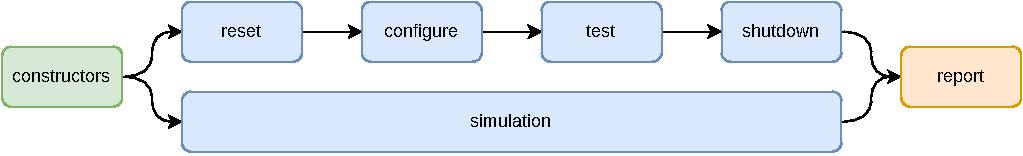
\includegraphics[width=\textwidth]{diagrams/own_phases.pdf}
  \caption{The simplified phasing system of the verification framework.}
  \label{fig:phases}
\end{figure}

The final phasing system is shown in Figure \ref{fig:phases}. The constructors are not an actual phase but are still
shown for clarity before the start of the run phases. The phase system is kept very simple, but it should, at least
for standard cases, provide the synchronization points necessary to structure the testbench execution.

One callenge a distributed testbench faces is the decision of when a phase has finished. In UVM, components can raise an objection, which that they are not yet ready to proceed to the next phase. They signal that they are done by dropping the objection. This way also a driver could for instance block the run phase from finishing until it has received its last response. In the verification framework a less powerful but simples approach is chosen. Components running code in the simulation phase have no way to object to the simulation finishing. Instead the reset, configure, test and shutdown phases finish once all participants have returned from the method associated with the phase. The simulation phase is thus meant for components which provide a static service in the testbench such as a driver or monitor. The reset, configure, test and shutdown phases are meant for components which \textit{control} the testbench in a fixed number of steps and exit once they are done. This way the simulation phase can be used to provide services to the testbench which are always available, while the other phases are used to control the testbench execution. 

An issue that the controlling phases have, is that some actions which they trigger may take an unpredictable time to finish. In this case, a controlling phase such as the test phase should interrogate service providing components such as drivers to determine when all its actions have taken effect. This could for instance be done by waiting for sequence to finish producing stimulus, or by waiting for a monitor to observe a certain number of transactions on an interface. 

\todo{when does this phase exit objection system NOT work?}



\begin{comment}
- core concept in UVM
- the use case for the runtime phases is to modularize the test phases such that they can be composed and overwritten
through inheritance
- argument for the build phases is not so clear
- why does the build phase have to be different from the constructor of a class?
- why does the connect phase first have to come thereafter
- build phase is top down -> makes sense since components instantiate their children
- connect phase is bottom up
- \cite{uvm_phases} says it is necessary to ensure that components exist before they are referenced and since they
can be created at any time, it is necessary to ensure that phases are followed
- but constructor is also a function not a task in SystemVerilog -> no time passes

- in a components contructor:
- it sets the parameters for the children
- it calls the constructors for the children
- it now has references to fully constructed and connected children
- it connects the children and exposes the interfaces of children

- this way a component is fully constructed and connected when the constructor finishes
- it is thus impossible to have a not fully initialized component hieararchy
- and it can be seen that the top down and bottom up approach still holds:
- the instances are created top down because a component is always created by its parent
- but the connections are done after all children have been constructed -> the leaf component connects first
- connect is rippling up before each contructor exits

- whatever a component needs to do should only affect itself and its children
- after the children have been constructed, they can be used
- so any setup before the simulation starts should be handled in the constructors of the components
- all build phases are replaced by the constructors

- what about inheritance?
- the constructor of the base class should always be called first in the constructor of the derived class to ensure
that all fields are initialized

- what about the extract, check, report and final?
- extract and check serve the purpose of preparing report
- why not let it be up to the one reporting how to prepare the report?
- if the argument is that it is better to compose using inheritance (if extract does not need to be overwritten but
check does...), why not let the user decide what function should be inherited
- in terms of necesssary synchronization for the components, only a report phase is necessary to ensure that all
components have finished their work
- no real concrete use case is given for final
- after report, nothing should be output, no sim is running, what should be left to do?

- this leaves us with the run time phases
- run phase is necessary for components like drivers to always be available to receive transactions
- all finer granularity run time phases seem to have their use case
- the pre and post ones not really
- as \cite[Ch. 4.6]{mehta2018asic} notes, not much use is anticipated for the pre and post run time phases
\end{comment}

\subsection{Reusable Verification Primitives} %--------------------------------------------------------------------------------

Providing a set of primitives and a standard manner of composing them is a key part of facilitating the reuse of
verification components. The verification framework will follow the recommendations of \citeauthor{sutherland2015uvm}
\cite{sutherland2015uvm} for a minimal UVM subset required for practical verification according to the UVM. The
primitives which are mentioned by the authors match with those generally presented in the literature. These base primitives are:

\begin{itemize}
  \item The sequence item: The transaction primitive
  \item The sequence: Generates transaction sequences
  \item The driver: Drives transactions on the DUT's ports
  \item The sequencer: Arbitrates multiple sequences' access to the driver
  \item The monitor: Observes the DUT's ports and publishes observed transactions
  \item The analysis component: Subscribes to transactions and performs analysis or checks
  \item The agent: Contains all components necessary for a single interface
  \item The environment: Contains agents and other components necessary for a (sub)system
  \item The test: Contains the top environment and controls stimulus generation
\end{itemize}

Each of these components has a distinct role in the static verification environment, as it has been outlined in
Chapter \ref{ch:background}. As such, each of them is needed to build a complete testbench, and the framework should
provide base classes for each of them which the user can extend.

In UVM these base components are implemented in a class hiearchy with \textit{uvm void} being the base class. Derived
from this is the \ttt{uvm\_object} which provides a series of features like printing, recording, copying, comparing
as well as packing and unpacking, i.e. serialization, of objects. The \textit{uvm report object} is derived from
this, adding logging funnctionality. The \textit{uvm component} base class is derived from the \textit{uvm report
object} and adds phasing, hierarchy tracking and the factory interface. UVM sequence items and sequences are derived
from the \textit{uvm object} class.

As noted by \citeauthor{sutherland2015uvm} \cite{sutherland2015uvm}, not all of this class hiearchy is relevant to
the end-user of UVM. In the framework, three base classes are provided: Components, Transactions and Sequences.
Instead of relying on inheritance to share functionality among these as it is done in the UVM, traits shall be used
to compose the required functionality of these primitives.

A Component is the base type for all the static elements of the testbench. It is hierarchy-aware by holding
references to its parent and children. Phasing is not a direct part of the Component base type. Instead, as it has
been discussed previously, phases are added to a component by adding traits to it. For instance a component can
execute code in the simulation phase by extending the \ttt{SimulationPhase} trait and implementing the \ttt{sim}
method. Components add logging capabilities with hierarchical awareness which will be further discussed in Section
\ref{sec:logging}.

The Transaction base type is used to capture the stimulus items which are sent to the DUT. For transactions it is
important to be able to check for data equality. This is done by implementing the \ttt{equivalent} method.
Furthermore, it is important to copy transactions, which is facilitated by implementing the \ttt{copy} method.
Serialization and recording of transactions is considered outside of the scope of the framework. The Sequence base
type is used to generate transactions. It's design will be considered in more detail in Section \ref{sec:stimulus_sequences}.

\begin{comment}

- in uvm all extend uvm\_object and then uvm\_component
- uvm obj provides
  - factory interface
  - printing -> toString
  - recording -> outside of scope
  - copying -> should be defined for transaction type
  - comparing -> case classes support it, but for general classes user has to define, Ordered[T] and Comparable[T] exist in scala
  - serdes -> outside of scope

-

\cite{sutherland2015uvm} -> what is a practical subset for UVM

- \cite{sutherland2015uvm} will be used as reference for which features are necessary for a practical verification framework
-

- things that are needed
- a test primitive
- an environment container primitive
- an agent primitive
- a sequencer primitive
- a driver primitive
- an monitor primitive
- an analysis component primitive (subscriber)
-

- a UVM testbench is close to a hdl test harness with static components

- do we actually need static components? why is the driver not just a function? transactors are just functions
mapping one abstraction level to another...
- the sequencer is just a generator, a thing we can get new values from, a driver is just a function, it is the test
case that should call the driver and let that code block until the transaction is done, or fork the interaction to continue

- the whole control flow surrounding sequences in the UVM seems weird
- a sequence aka generator should be passed to a sequencer, which should run in its own thread and generate
transactions on the driver port pulling from different incomin sequences aka a channel mux in gears
\end{comment}

\subsection{Stimulus Sequences} %----------------------------------------------------------------------------------------------
\label{sec:stimulus_sequences}

Sequences are a necessary mechanism to structure the generation of stimulus such that it can be reused and composed.
The UVM design of sequences is quite straight forward and easy to use. All the user has to do is implement the
\ttt{body} method in which items can be generated. The communication with the receiver of the produced items is done
through the \ttt{start\_item} and \ttt{finish\_item} methods. The \ttt{start\_item} call blocks until the sequencer
grants the sequence the right to produce an item, while the \ttt{finish\_item} call actually sends the item and wait
for the response from the receiver.

In the verification framework, the syntax should orient itself more towards generators. In F\# for instance, a new
item in a sequence is produced calling \ttt{yield item}, while a sequence of items can be produced one after the
other using \ttt{yield! seq}. For the framework, a call to \ttt{yieldTx(tx)} shall produce the item, and return
the response item of a possibly different type. This means only a single function call is necessary to produce an item and receive the response.
Other sequences can be added to the stream of the sequence using \ttt{yieldSeq(seq)} which forward the items of that sequence and provide it with the received responses.

It is not always necessary to use a generator to produce stimulus. The advantage of the generator is that it can have a complex stateful behavior which is captured the code of its body. If simple sequences, like for instance a fixed-length sequence of random items, are needed, standard Scala collections should be used. For instance the \ttt{Seq.fill(n)(fun)} function can be used to generate a sequence of \ttt{n} items by calling the \ttt{fun} function \ttt{n} times. The \ttt{Seq.tabulate(n)(i => fun(i))} function can be used to generate a sequence of \ttt{n} items by providing the function \ttt{fun} with the index of the item. In order to allow for the composing of Scala collections and sequences, \ttt{yieldSeq} also should accept a Scala collection as an argument. Furthermore, a Scala collection can be converted to a sequence using the \ttt{.toSequence} method. An example of a sequence is shown in Listing \ref{lst:sequence}. Two items are produced using the \ttt{yieldTx} method, while two more items are produced using a scala \ttt{Seq} collection.


Sequences can be composed by creating a new sequences which coordinates the execution of multiple sequences. In the case of a simple composition, standard operators should be provided to compose sequences. Some ideas for sequence combinators are:

\begin{itemize}
  \item \ttt{Sequence.concat(a,b,..)}: Concatenate sequences \ttt{a}, \ttt{b}, ...
  \item \ttt{Sequence.interleave(a,b)}: Interleave two sequences \ttt{a} and \ttt{b}
  \item \ttt{Sequence.mix(a,b)}: Randomly forward items from either sequence \ttt{a} or \ttt{b}
  \item \ttt{Sequence.repeat(a,n)}: Repeat sequence \ttt{a} \ttt{n} times
  \item \ttt{Sequence.map(a,f)}: Apply function \ttt{f} to each item of sequence \ttt{a}
  \item \ttt{Sequence.filter(a,p)}: Filter items of sequence \ttt{a} using predicate \ttt{p}
\end{itemize}

Some of these operators like \ttt{map} and \ttt{filter} take inspiration from common functional programming higher-order functions.


\begin{listing}
\begin{lstlisting}[language=scala, captionpos=b, caption=Example of a sequence producing four items of type \ttt{Tx} with responses of type \ttt{Resp}.,label=lst:sequence]
class MySeq extends Sequence[Tx, Resp] {
  def body: Unit = {
    val r0 = yieldTx(new Tx(0))
    val r1 = yieldTx(new Tx(1))
    val s = Seq.tabulate(2)(i => new Tx(i + 2))
    val Seq(r2, r3) = yieldSeq(s)
  }
}
\end{lstlisting}
\end{listing}

To actually use a sequence, it has to be handed of to a sequencer. In the framework, a simple sequencer shall be provided which plays one sequence after the other on a first-come-first-served basis. A sequence is played by calling the method \ttt{sequencer.play(seq)}. The call blocks until the sequencer is ready to start palying the sequence.

Often, it is of interest for a test case to know when a sequence has finished, i.e. all items have been handed off to the driver and the responses have been received. This can be done by calling the \ttt{seq.waitUntilDone()} method which blocks until the sequence has finished.

\begin{comment}
  
- scala sequences should be convertable to sequences

\todo{what about virtual sequences}
- virtual sequences are about targetting different sequencers
- could yieldItem(seq, item) be used to target a different sequencer?

- sequences are a necessary mechanism to structure the generation of stimulus
- their implementation in UVM is quite good
- a sequence is a generator of transactions
- it is not clear why sequence needs two methods: start and finish item
- a sequence should prepare an item, then yield it
- the call to yield should return the response item
\end{comment}


\subsection{Running a Test} %-----------------------------------------------------------------------------------------------

In order to run a test case which the user has written, it has to be handed to a runtime which executes the different
phases. This is handled by the \ttt{runTest} function. It takes takes an instance of the DUT's interface and a
closure to create the test case. The closure receives the DUT instance as an argument. If case the testcase expects a
BFM instead of the direct interface to the DUT, the user can construct it in the closure before returning the test
instance. The \ttt{runTest} function retunrs once the test is finished. An example of how to run a test is shown in
Listing \ref{lst:runTest}.

\begin{listing}
\begin{lstlisting}[language=scala, captionpos=b, caption=Example code for running a test case using the verification framework.,label=lst:runTest]
runTest(new MyDUT) { dut =>
  new MyTest(dut)
}
\end{lstlisting}
\end{listing}

In addition to complex UVM-style testbenches, the framework should also support simpler tests. The Chiseltest
framework provides a simple way to write unit-test-like directed tests in a concise manner. These purely rely on the
peek, poke and expect functions or a BFM to interact with the DUT. This should also be possible in the verification
framework. The \ttt{Simulation} function is provided for this purpose. It takes the DUT instance and a closure which
contains the test code. An example is shown in Listing \ref{lst:unitTest}.

\begin{listing}
\begin{lstlisting}[language=scala, captionpos=b, caption=Example code for running a test case using the verification framework.,label=lst:unitTest]
Simulation(new MyDUT) { dut =>
  poke(dut.a, 1)
  poke(dut.b, 2)
  dut.clk.step(1)
  dut.c.except(3)
}
\end{lstlisting}
\end{listing}

\subsection{Testbench Configurability} %---------------------------------------------------------------------------------------

UVM requires a recompilation for each testbench \cite{salemi2013uvm}, we do not need that since a jar can have
multiple entry points.

\todo{consider callbacks -> in scala easy to implement with higher order functions}

- alternative to factory could be dependency injection
- an agent receives its driver through a parameter
- driver is of certain trait or class or a derivative thereof

- configDB should not require error handling all the time, throw exception on miss and have try method
- else parameters as class parameters for components
- causes problem with factory, since factory instantiation only accepts name, else varargs but that is not compile time checked

- static hierarchy, and we want to switch out components -> need to anticipate switch
- why not do dependency injection? then the compiler will help us guarantee that the switch works
- this causes problem with UVM

- if the factory is used, we could pass a small config db to the factory
- each component should then specify its parameters such that the factory checks automatically if all paramters are defined

\subsection{Logging} %---------------------------------------------------------------------------------------------------------
\label{sec:logging}

For debugging puporses it is important to have a logging system. Here the UVM provides a powerful logging system
which tags messages by the component that has issued it. This allows for filtering of messages by component. In
addition the UVM provides verbosity levels to control how detailed the logging should be.

In the verification framework, a similar logging system should be available. The component base type should provide
functions for printing info, warning and error messages. In addition to tagging these messages with the components
hierarchical name, source file and line number information should be added to give a pointer to where the message was
issued in the code. The functionality of fatal errors in UVM is not necessary, since the Scala exception system can
be used instead.

\subsection{Register Abstraction} %--------------------------------------------------------------------------------------------

\subsection{Functional Coverage} %---------------------------------------------------------------------------------------------

- functional coverage

- coverage groupps can be hieararchy aware!

\begin{lstlisting}
class MyGroup extends CoverGroup {
  val a = coverpoint(a) {
    bin("a0", 0 until 10)
    bin("a1", 10 until 20)
  }
  coverpoint(b) {
    bin("b0", 0 until 10)
    bin("b1", 10 until 20)
  }
}
\end{lstlisting}

functional coverage should be able to collect coverage for scala values! transactions are where coverage is measured

a covergroup with its sampling event should be passed to verification runtime

\subsection{Constrained-Random Stimuli Generation} %---------------------------------------------------------------------------

- variable types
- support not only for hardware types but scala types
- bitvector types
- integer types
- floating point types
- enumeration types
- string type?
- randomize with constraints

- for signal processing purposes it may be interesting to have a continuous random signal i.e. a random walk

\subsection{Debugging} %-------------------------------------------------------------------------------------------------------
\todo{interactive tests? the scala repl could be used}


\chapter{Implementation} %/////////////////////////////////////////////////////////////////////////////////////////////////////

\section{Simulation Runtime} %=================================================================================================

\subsection{Interfacing the Verilated Model} %---------------------------------------------------------------------------------

Verilator transpiles the SystemVerilog source code into a C++ class. A mechanism is needed by which the Scala test code can interact with an instance of this class. The JNA (java native access) library can be used to call native functions from the java virtual machine (JVM). In C++, a simulation context class is used to keep all required objects. The following set of functions is provided, which take the simulation context as an argument to interact with the simulation:


\begin{itemize}
  \item \ttt{createSimContext\_XX} creates a new simulation context and return a pointer to it
  \item \ttt{destroySimContext\_XX} destroys a simulation context
  \item \ttt{setInput\_XX} sets the value of the input signal mapped to the provided id
  \item \ttt{setInputWide\_XX} sets the value of the input signal mapped to the provided id for inputs wider than 64 bits
  \item \ttt{getOutput\_XX} gets the value of the output signal mapped to the provided id
  \item \ttt{getOutputWide\_XX} gets the value of the output signal mapped to the provided id for outputs wider than 64 bits
  \item \ttt{tick\_XX} evaluates the model and advances the simulation by one clock cycle
\end{itemize}

The functions are suffixed with the name of the top-level module (signified by \ttt{\_XX}) to make them unique, allowing for multiple models to be loaded into the same JVM instance. The simulation context and functions are compiled together with the Verilator model into a shared library which can be loaded by the JNA library at runtime. A Makefile is generated alongside the model specific simulation interface functions in the Scala code before a simulation is started. The usage of a Makefile results in the shared library to be recompiled only when the model changes.
  

\todo{mention somewhere that an attempt for register access was successfully made}

\subsection{Concurrency} %----------------------------------------------------------------------------------------------



- threads are an option but have a lot of overhead, each their own stack
- in cocotb coroutines are used 
- project loom adds green threads to the JVM \cite{loom}
- a new library in scala 3 by epfl called gears tries to take advantage for async style programming \cite{gears}
- uses scalas context parameters: functions use context dependent values 
- async functions take async context as parameter def myfun(...)(using Async)
- this allows for structured concurrency -> a newly spawned thread knows about its parent 
- well suited for fork-join model

\subsection{Simulation Controller} %-------------------------------------------------------------------------------------------

- accesses to the simulation have to be serialized
- either lock for simulation
- but who has responsibility to drive the simulation after all threads sleep?
- could be the last thread which sleeps
- instead a model is chosen where a simulation controller runs and receives commands from the simulation threads through a channel
- channel serializes commands
- simulation threads issue request and wait to be waken up or receive an answer by waiting for a response on another channel
- commands:
  - register thread
  - deregister thread
  - poke
  - peek
  - step
  - Mark
  - SentToChannel
  - WaitForChannel
  - WaitForThread
  - finish
  - Abort

- sim controller needs to know all simulation threads and keep track of their status
- therefore register and deregister commands are necessary

- sim controller keeps an event queue
- the following events exist
  - Drive
  - PosEdge
  - NegEdge
  - release

- pokes create a drive event at the falling edge of their clock domain
- peeks are served immediately
- clock events schedule the next edge when they are executed

- step command schedules a release event for the appropriate time
- once all threads sleep, the controller advances to the next time with an event, executes all events
- if threads are released, the controller waits for thm to finish before advancing to the next time

- since channel communication may put threads to sleep while waiting (i.e. sim is allowed to advance) the channel communication has to happen through the sim controller
- join mechanism is the same

- finish command for good exit
- abort command for bad exit

- question is now how to give threads access to sim controller
- global means only a single sim instance
- dynamic variable would be solution
- but since Async uses context parameters -> Sim context parameter is used
- as such function which use the simulation controller def myfun(...)(using Sim, Async) 
- async is needed since interaction with sim may put thread to sleep

- the actual functions to interact with the simulation are extensions to the port types
- they use the Sim context to send the appropriate command to the simulation controller
- example in Listing \ref{lst:simctx}
- simcontext is provided in sim closure as context parameters

\begin{listing}
\begin{lstlisting}[language=scala, captionpos=b, caption=Example code for a function using the simulation context to interact with a DUT.,label=lst:simctx]
def add(dut: Adder)(a: Int, b: Int)
                   (using Sim, Async): Unit = {
  dut.a.poke(a)
  dut.b.poke(b)
  dut.clk.step(1)
  dut.c.expect(a + b)
}

Simulation(new Adder) { dut =>
  add(dut)(1, 2)
}
\end{lstlisting}
\end{listing}

\section{Verification Environment} %===========================================================================================

\subsection{Phases} %----------------------------------------------------------------------------------------------------------

- like it was discussed earlier, phases are implemented as traits
- a component can implement multiple phases by extending multiple traits
- each trait comes with one function which is called in the phase
- a function taking the root component as argument exists for every phase
- it starts up forks for simulation phases and else just calls the function
- whether a component implements a phase is easily determined by a pattern match on the trait
- inside the runTest the phases are called in order on the root components

\subsection{Component Hierarchy} %---------------------------------------------------------------------------------------------

\subsection{Inter-Component Communication} %-----------------------------------------------------------------------------------

\subsection{Component Configuration} %-----------------------------------------------------------------------------------------

\subsection{Stimulus and Sequences} %-------------------------------------------------------------------------------------------

\subsection{Test Cases} %------------------------------------------------------------------------------------------------------

\subsection{Register Abstraction} %--------------------------------------------------------------------------------------------

\chapter{Results} %////////////////////////////////////////////////////////////////////////////////////////////////////////////

\section{Use-Cases} %----------------------------------------------------------------------------------------------------------

\subsection{Use-Case 1: Simple ALU} %------------------------------------------------------------------------------------------

\subsection{Use-Case 2: Memory-Mapped UART} %----------------------------------------------------------------------------------

\subsection{Use-Case 3: APB Verification IP} %---------------------------------------------------------------------------------

\section{Performance} %--------------------------------------------------------------------------------------------------------

\chapter{Discussion} %/////////////////////////////////////////////////////////////////////////////////////////////////////////

- scala 3 was chosen to use newest features and make future proof but that prevents integration with chisel

- annoying to write interface in scala and SystemVerilog -> simple tool could create scala code from SystemVerilog

- it is really difficult working with something which is promised to bear fruit for really complex cases when time is
limited and does not allow for creating cases which would show the full potential
- I also don't have the use case and expertise to showcase full blown UVM
- the design of such a framework should build on actual experience with large verification projects

%\section{Future Work} %========================================================================================================

- verilator performance features (multi-threading, ...)

- allow for setting top level verilog parameters

- add support for attached models
- a function receiving the dut and can do whatever it likes, reading outputs, setting inputs to for instance model a
UART/SPI/Memory
- simulation loop could call the function in each evaluation step

- integration with scalatest

\chapter{Conclusion} %/////////////////////////////////////////////////////////////////////////////////////////////////////////

\printbibliography

\end{document}

\section{Hardware Description Languages}

\section{Hardware Verification Languages}

\section{Concurrency Models}
- talk about how HDL concurrency models differ from other
- talk about other concurrency models
- is UVM actor based?

\subsection{Superlog}

\citeauthor{flake2020a} \cite[Sec. 6, pp. 44-49]{flake2020a}
- engineers at Co-Design Automation Inc. saw potential in conciseness and closeness to HW in Verilog
- C was chosen as a source of inspiration for language extensions due to wide spread use in EDA and embedded systems
communitites
- this turned into superlog
- additions included:
- variable size data types (queues, sparse arrays, associative arrays)
- bundled data types with different directions
- enumerations
- references
- C dpi
- interfaces as collection of wires, but also exposing of methods of modules without hierarchical references

-

\section{UVM}

\section{Transaction-Level Modeling}

\section{Software Testing Methods}
- unit testing
- integration testing
- system testing
- black vs. grey vs. white box testing
